%initialising document, adjust papersize, fontsize and page orientation to your needs
\documentclass[a4paper, fontsize = 8pt, landscape]{scrartcl}
\usepackage{../../../misc_files/LateX/layout_and_colours}
\makeatletter
\def\input@path{{content/LONG_summary/}{content/examples/}}
\makeatother

\graphicspath{{content/}{content/LONG_summary/}{content/examples/}}

\title{Software Entwicklung 1}
\author{Jil Zerndt, Lucien Perret}
\date{January 2025}

\createtitlepagestyle
\createmainpagestyle
\begin{document}
\begin{multicols}{3}
	\thispagestyle{TitlePageStyle}
	\maketitle
	\sffamily
	


\section{Overview of IT Security}

\mult{2}

\begin{definition}{Key IT Security Goals}
Information security is based on three fundamental principles, commonly known as the CIA triad:
\begin{itemize}
    \item \textbf{Confidentiality} - Ensuring data is only accessible to authorized users
    \item \textbf{Integrity} - Ensuring data is not modified in an unauthorized way
    \item \textbf{Availability} - Ensuring systems and data are accessible when needed
\end{itemize}
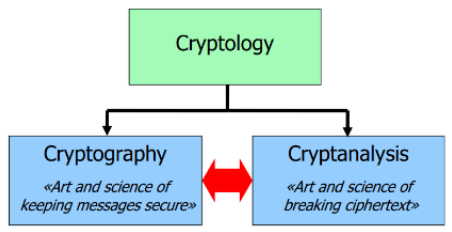
\includegraphics[width=0.6\linewidth]{its_goals.png}
\end{definition}

\begin{concept}{Business IT Risks}
\begin{itemize}
    \item Data loss
    \item System outage
    \item Espionage
    \item Sabotage
    \item Reputation loss
    \item Misuse of computing resources
    \item Violation of regulations
    \item Fraud
    \item Brand misuse
    \item Ransom demands
\end{itemize}
These risks can have significant financial, operational, and reputational impacts.
\end{concept}

\multend

\raggedcolumns

\subsubsection{Security Frameworks and Controls}

\mult{2}

\begin{concept}{Security Control Frameworks}
Security frameworks provide structured approaches to implementing security controls:
\begin{itemize}
    \item \textbf{CIS Controls} - Prioritized set of actions to protect organizations
    \item Controls are typically organized in implementation groups based on difficulty and impact
    \item Focus on preventing the most common attack vectors first
\end{itemize}
\end{concept}

\begin{definition}{Types of Security Measures}
Security measures can be categorized based on their focus:
\begin{itemize}
    \item \textbf{Preventive} - Block threats before they occur (firewalls, access controls)
    \item \textbf{Detective} - Identify when a breach has occurred (IDS, audit logs)
    \item \textbf{Corrective} - Mitigate damage after an incident (backups, incident response)
\end{itemize}
\end{definition}

\multend

\subsubsection{Disaster Recovery}



\begin{concept}{Business Continuity Management}
Disaster recovery and business continuity planning are essential for maintaining availability:
\begin{itemize}
    \item \textbf{Recovery Plan} - Detailed procedures for recovering from incidents
    \item \textbf{Recovery Tests} - Regular testing of recovery procedures
    \item \textbf{Redundancy} - Duplicate systems, power supplies, and network connections
    \item \textbf{Offline backups} - Protection against ransomware and other threats
\end{itemize}
\end{concept}

\begin{KR}{Disaster Recovery Planning}
\paragraph{Initial Assessment}
\begin{itemize}
    \item Identify critical systems and data
    \item Determine acceptable recovery time objectives (RTO)
    \item Determine acceptable recovery point objectives (RPO)
\end{itemize}

\paragraph{Plan Development}
\begin{itemize}
    \item Document recovery procedures
    \item Assign roles and responsibilities
    \item Include contact details for all relevant parties
    \item Develop technical instructions for restoration
\end{itemize}

\paragraph{Testing}
\begin{itemize}
    \item Conduct regular theoretical dry runs
    \item Perform practical tests (e.g., server shutdown, data restoration)
    \item Update procedures based on test results
\end{itemize}

\paragraph{Regular Review}
\begin{itemize}
    \item Review and update plans regularly
    \item Consider changes in infrastructure, personnel, and threats
\end{itemize}
\end{KR}

\begin{example}
A medium-sized company implements a disaster recovery plan for their customer database. They define an RTO of 4 hours and an RPO of 15 minutes, meaning they need to restore service within 4 hours with no more than 15 minutes of data loss. To achieve this, they implement a combination of hourly differential backups with continuous transaction log shipping to a standby site. Regular recovery tests are scheduled quarterly to ensure the plan remains effective.
\end{example}

\mult{2}


\begin{concept}{Problems - Overview}\\ and their impact on data availability
\paragraph{Physisch}
\textbf{unabsichtlich}
\begin{itemize}
    \item Naturkatastrophen
    \item Feuer
    \item Ausfall
    \item Kaffee auf Server
\end{itemize}

\textbf{absichtlich/bösartig}
\begin{itemize}
    \item Feuer
    \item Vandalismus
    \item Garantie läuft aus -> absichtlich langsamer
    \item Social Engineering
\end{itemize}

\paragraph{Virtuell}
\textbf{unabsichtlich}
\begin{itemize}
    \item Bitflip
    \item Config Fehler
    \item Bugs im SW
    \item Phishing klicken
\end{itemize}

\textbf{absichtlich/bösartig}
\begin{itemize}
    \item DDoS
    \item Malware
    \item Ransomware
    \item Phishing senden
    \item Trojaner
\end{itemize}
\end{concept}

\begin{theorem}{Countermeasures - Overview}

\textbf{Disaster Recovery}
    \begin{itemize}
        \item Offline backup solutions
        \item Restoring from images
    \end{itemize}

\textbf{Access Control}
    \begin{itemize}
        \item Restricted Access Rights
        \item Multi-Factor Authentication
        \item Firewalls
        \item Traffic Management Solutions
    \end{itemize}

\textbf{Physical Protection}
    \begin{itemize}
        \item Physical Access Control (locks, fences, etc.)
        \item Fire Protection (extinguishers, alarms, etc.)
        \item Monitoring (CCTV, Guards etc.)
    \end{itemize}

\textbf{Training Processes}
    \begin{itemize}
        \item Employee Training
        \item Four eyes principle
        \item Automation of routine processes
        \item Monitoring
        \item Preventive maintenance
    \end{itemize}

\textbf{Redundancy}
    \begin{itemize}
        \item Uninterruptable Power Supplies
        \item High Availability setups
        \item Load Balancing
        \item Redundant data center
        \item Redundant network connections
    \end{itemize}
\end{theorem}

\multend

\mult{2}

\begin{formula}{Recovery Plan and Test}

    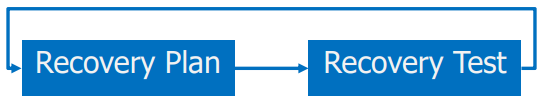
\includegraphics[width=0.7\linewidth]{recovery_plan_test.png}

    \textbf{Recovery Plan} - description of what to do if something goes wrong
    \begin{itemize}
        \item Roles and responsibilities
        \item Processes
        \item Contact details
        \item Technical instructions
    \end{itemize}

    \textbf{Recovery Test} - testing the recovery plan
    \begin{itemize}
        \item Theoretical dry run
        \item Practical tests
        \begin{itemize}
            \item turn off a server or DC
            \item restore data from backup
        \end{itemize}
    \end{itemize}
\end{formula}

\begin{concept}{Goals of IT Security}

Most measures in Information Security have one of the three following high-level goals:
\begin{itemize}
    \item Ensure data is confidential
    \item Ensure data is not corrupted
    \item Ensure data and systems are available
\end{itemize}

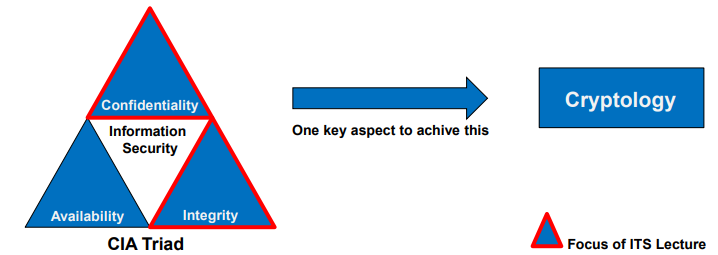
\includegraphics[width=\linewidth]{goals_of_IT_security.png}
\end{concept}

\multend

\raggedcolumns





	\raggedcolumns
	\pagebreak
	\section{Anforderungsanalyse}

\begin{definition}{Software Engineering}
\begin{itemize}
    \item \textbf{Disziplinen:} 
    Anforderungen, Architektur, Implementierung, Test und Wartung
    \item \textbf{Ziel:}  
    Strukturierte Prozesse für Qualität, Risiko- \& Fehlerminimierung
\end{itemize}
\end{definition} 

\subsection{Usability und User Experience}

\begin{concept}{Usability und User Experience} drei Säulen der Benutzererfahrung:
    \begin{itemize}
        \item \textbf{Usability (Gebrauchstauglichkeit):} \\ Grundlegende Nutzbarkeit des Systems
        \item \textbf{User Experience:} Usability + Desirability (Attraktivität)
        \item \textbf{Customer Experience:} \\ UX + Brand Experience (Markenwahrnehmung)
    \end{itemize}
    %todo: better resolution image
    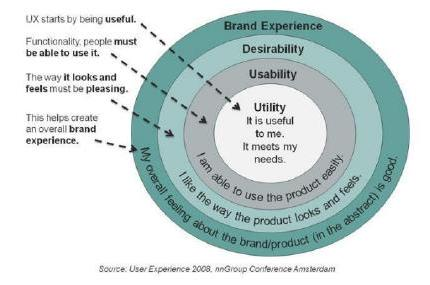
\includegraphics[width=0.6\linewidth]{images/2024_12_29_0d1d7b5551ea1b4b41bdg-02}
    
    \textbf{Wichtige Aspekte:}
    Benutzer und seine Ziele/Aufgaben, Kontext der Nutzung, Softwaresystem (inkl. UI)
\end{concept}

\begin{definition}{Usability-Dimensionen nach ISO 9241}
\begin{itemize}
    \item \textbf{Effektivität:}
    \begin{itemize}
        \item Der Benutzer kann alle Aufgaben vollständig erfüllen
        \item Gewünschte Genauigkeit wird erreicht
        \item Ziele werden im vorgegebenen Kontext erreicht
    \end{itemize}
    \end{itemize}

\begin{minipage}{0.5\linewidth}
    \begin{itemize}
    \item \textbf{Effizienz:} \\ Minimaler Aufwand für:
    \begin{itemize}
        \item Mentale Belastung
        \item Physische Anstrengung
        \item Zeitlicher Aufwand
        \item Ressourceneinsatz
    \end{itemize}
    \end{itemize}
\end{minipage}
\begin{minipage}{0.5\linewidth}
    \begin{itemize}
    \item \textbf{Zufriedenheit:}
    \begin{itemize}
        \item Minimum: Keine Verärgerung
        \item Standard: Zufriedenheit
        \item Optimal: Begeisterung
        \item Subjektive Nutzererfahrung
    \end{itemize}
\end{itemize}
\end{minipage}
\end{definition}

\begin{KR}{Usability-Evaluation durchführen}
\vspace{-2mm}\\
\begin{minipage}[t]{0.5\linewidth}
\begin{enumerate}[start=1]
    \item \textbf{Vorbereitung}
    \begin{itemize}
        \item Testziele definieren
        \item Testpersonen auswählen
        \item Testaufgaben erstellen
    \end{itemize}
    \item \textbf{Durchführung}
    \begin{itemize}
        \item Beobachtung der Nutzer
        \item Protokollierung von \\Problemen
        \item Zeitmessung der Aufgaben
    \end{itemize}
\end{enumerate}
\end{minipage}
\begin{minipage}[t]{0.5\linewidth}
\begin{enumerate}[start=3]
    \item \textbf{Auswertung}
    \begin{itemize}
        \item Probleme klassifizieren
        \item Schweregrad bestimmen
        \item Verbesserungen vorschlagen
    \end{itemize}
    
    \item \textbf{Dokumentation}
    \begin{itemize}
        \item Ergebnisse zusammenfassen
        \item Empfehlungen formulieren
        \item Maßnahmen priorisieren
    \end{itemize}
\end{enumerate}
\end{minipage}
\end{KR}

\begin{theorem}{ISO 9241-110: Usability-Anforderungen}

\begin{minipage}[t]{0.58\linewidth}
\begin{itemize}
    \item \textbf{Aufgabenangemessenheit:}
    \begin{itemize}
        \item Funktionalität unterstützt \\ Arbeitsaufgaben
        \item Keine unnötige Komplexität
    \end{itemize}
    
    \item \textbf{Selbstbeschreibungsfähigkeit:}
    \begin{itemize}
        \item Verständliche Benutzerführung
        \item Klare Statusanzeigen
    \end{itemize}
    
    \item \textbf{Steuerbarkeit:}
    \begin{itemize}
        \item Benutzer kontrolliert Ablauf
        \item Geschwindigkeit anpassbar
    \end{itemize}
    
    \item \textbf{Erwartungskonformität:}
    \begin{itemize}
        \item Konsistentes Verhalten
        \item Bekannte Konventionen
    \end{itemize}
\end{itemize}
\end{minipage}
\begin{minipage}[t]{0.4\linewidth}
\begin{itemize}    
    \item \textbf{Fehlertoleranz:}
    \begin{itemize}
        \item Fehler vermeiden
        \item Fehlerkorrektur \\ ermöglichen
    \end{itemize}
    
    \item \textbf{Individualisierbarkeit:}
    \begin{itemize}
        \item Anpassung an \\ Benutzergruppen
        \item Flexible Nutzung
    \end{itemize}
    
    \item \textbf{Lernförderlichkeit:}
    \begin{itemize}
        \item Einfacher Einstieg
        \item Unterstützung beim \\ Lernen
    \end{itemize}
\end{itemize}
\end{minipage}
\end{theorem}

\subsection{User-Centered Design (UCD)}

\begin{concept}{UCD Prozess}

\begin{minipage}{0.4\linewidth}
Ein iterativer Prozess zur nutzerzentrierten \\ Entwicklung, der die Bedürfnisse, Wünsche und Einschränkungen 
der Benutzer in jeder Phase des Design-Prozesses berücksichtigt.

\textbf{Hauptziele:}
\begin{itemize}
    \item Benutzerfreundlichkeit
    \item Effektive Nutzung
    \item Hohe Akzeptanz
\end{itemize}
\end{minipage}
\begin{minipage}{0.6\linewidth}
    \vspace{-5mm}
    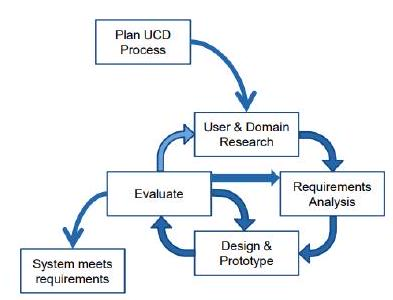
\includegraphics[width=\linewidth]{images/2024_12_29_0d1d7b5551ea1b4b41bdg-03}
\end{minipage}
\end{concept}

\begin{corollary}{Wichtige Artefakte}
\begin{itemize}
    \item Personas: Repräsentative Nutzerprofile
    \item Usage-Szenarien: Konkrete Anwendungsfälle
    \item Mentales Modell: Nutzerverständnis
    \item Domänenmodell: Fachliches Verständnis
    \item Service Blueprint: Geschäftsprozessmodell
    \item Stakeholder Map: Beteiligte und Betroffene
    \item UI-Artefakte: Skizzen, Wireframes, Designs
\end{itemize}
\end{corollary}

\begin{example2}{Stakeholder Map}\\
Zeigt die wichtigsten Stakeholder im Umfeld der Problemdomäne.\\
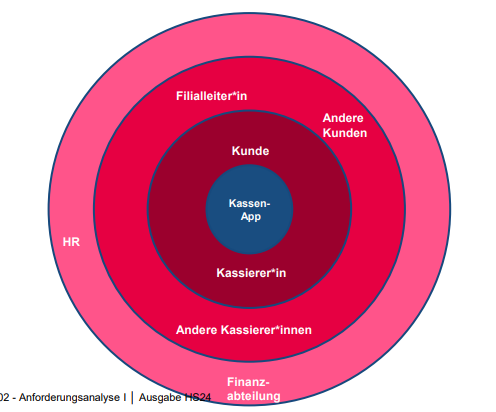
\includegraphics[width=0.8\linewidth]{images/stakeholdermap.png}
\end{example2}



\begin{theorem}{UCD Prozess-Phasen}\\
\textbf{1. User \& Domain Research} (see KR)

\textbf{2. Requirements Analysis} (see KR)

\begin{minipage}[t]{0.5\linewidth}
\textbf{3. Design \& Prototype}
\begin{itemize}
    \item Interaktionskonzept entwickeln
    \item Wireframes erstellen
    \item Prototypen bauen
    \item Design iterativ verbessern
\end{itemize}
\end{minipage}
\begin{minipage}[t]{0.5\linewidth}
\textbf{4. Evaluate}
\begin{itemize}
    \item Mit Benutzern testen
    \item Feedback sammeln
    \item Probleme identifizieren
    \item Verbesserungen einarbeiten
\end{itemize}
\end{minipage}
\end{theorem}

\begin{KR}{User \& Domain Research}
\begin{enumerate}
    \item \textbf{Zielgruppe identifizieren}
    \begin{itemize}
        \item Wer sind die Benutzer?
        \item Was sind ihre Aufgaben/Ziele?
        \item Wie sieht ihre Arbeitsumgebung aus?
        \item Welche Sprache/Begriffe verwenden sie?
    \end{itemize}
\end{enumerate}

\begin{minipage}[t]{0.5\linewidth}
\begin{enumerate}[start=2]
    \item \textbf{Daten sammeln durch}
    \begin{itemize}
        \item Contextual Inquiry
        \item Interviews
        \item Beobachtung
        \item Fokusgruppen
        \item Nutzungsauswertung
    \end{itemize}
\end{enumerate}
\end{minipage}
\begin{minipage}[t]{0.5\linewidth}
\begin{enumerate}[start=3]
    \item \textbf{Ergebnisse dokumentieren in}
    \begin{itemize}
        \item Personas
        \item Usage-Szenarien
        \item Mentales Modell
    \end{itemize}
\end{enumerate}
\end{minipage}
\end{KR}

\begin{KR}{UCD Artefakte erstellen}

\begin{minipage}[t]{0.45\linewidth}
\textbf{1. Personas}
\begin{itemize}
    \item Daten aus User Research\\ sammeln
    \item Gemeinsame Merkmale \\identifizieren
    \item Repräsentative Person \\definieren
    \item Details ausarbeiten:
    \begin{itemize}
        \item Demografische Daten
        \item Ziele und Motivation
        \item Fähigkeiten/Kenntnisse
        \item Frustrationspunkte
    \end{itemize}
\end{itemize}
\end{minipage}
\begin{minipage}[t]{0.5\linewidth}
\textbf{2. Usage-Szenarien}
\begin{itemize}
    \item Kontext beschreiben
    \item Akteure identifizieren
    \item Ablauf definieren
    \item Probleme/Lösungen darstellen
\end{itemize}

\textbf{3. Mentales Modell}
\begin{itemize}
    \item Nutzerverständnis\\ dokumentieren
    \item Konzepte und Beziehungen \\visualisieren
    \item Mit Fachmodell abgleichen
\end{itemize}
\end{minipage}
\end{KR}

\begin{example2}{Usage-Szenario: Online-Banking}\\
\textbf{Kontext:} Sarah möchte eine Überweisung tätigen

\textbf{Aktuelles Szenario:}
Sarah loggt sich in ihr Online-Banking ein. Sie sucht nach der letzten Überweisung an ihren Vermieter, um die Kontodetails zu finden. Nach mehreren Klicks findet sie die Information und kopiert die IBAN. Sie öffnet das Überweisungsformular und fügt die Daten ein. Beim Absenden erscheint eine Fehlermeldung, weil sie vergessen hat, den Verwendungszweck einzutragen.

\textbf{Probleme:}
\begin{itemize}
    \item Umständliche Suche nach Kontodetails
    \item Fehleranfällige manuelle Dateneingabe
    \item Späte Validierung der Eingaben
\end{itemize}

\textbf{Verbessertes Szenario:}
Sarah wählt aus einer Liste ihrer häufigen Empfänger ihren Vermieter aus. Das System füllt automatisch alle bekannten Daten ein. Fehlende Pflichtfelder sind deutlich markiert. Sarah ergänzt den Verwendungszweck und sendet die Überweisung ab.
\end{example2}

\begin{remark}
    Weitere Beispiele z.B. Persona erstellen auf nächster Seite
\end{remark}

\begin{example2}{Persona erstellen}\\
\textbf{Aufgabe:} Erstellen Sie eine Persona für ein Online-Banking-System.

\textbf{Lösung:} 
\textbf{Sarah Schmidt, 34, Projektmanagerin}
\begin{itemize}
    \item \textbf{Hintergrund:}
    \begin{itemize}
        \item Arbeitet Vollzeit in IT-Firma
        \item Technik-affin, aber keine Expertin
        \item Nutzt Smartphone für die meisten Aufgaben
    \end{itemize}
    \item \textbf{Ziele:}
    \begin{itemize}
        \item Schnelle Überweisungen zwischen Konten
        \item Überblick über Ausgaben
        \item Sichere Authentifizierung
    \end{itemize}
    \item \textbf{Frustrationen:}
    \begin{itemize}
        \item Komplexe Menüführung
        \item Lange Ladezeiten
        \item Mehrfache Login-Prozesse
    \end{itemize}
\end{itemize}
\end{example2}

\begin{example2}{Persona für E-Learning-System}\\
\textbf{Thomas Weber, 19, Informatik-Student}

\textbf{Hintergrund:}
\begin{itemize}
    \item Erstsemester-Student
    \item Arbeitet nebenbei 10h/Woche
    \item Pendelt zur Universität (1h pro Weg)
\end{itemize}

\textbf{Technische Fähigkeiten:}
\begin{itemize}
    \item Versiert im Umgang mit Computern
    \item Nutzt hauptsächlich Smartphone für Online-Aktivitäten
    \item Kennt gängige Learning-Management-Systeme
\end{itemize}

\textbf{Ziele:}
\begin{itemize}
    \item Effizientes Lernen trotz Zeitdruck
    \item Flexible Zugriffsmöglichkeiten auf Lernmaterialien
    \item Gute Prüfungsvorbereitung
\end{itemize}

\textbf{Frustrationen:}
\begin{itemize}
    \item Unübersichtliche Kursstrukturen
    \item Fehlende Mobile-Optimierung
    \item Schwierige Navigation zwischen Materialien
\end{itemize}
\end{example2}

\subsection{Requirements Engineering}

\begin{definition}{Requirements (Anforderungen)}
\begin{itemize}
    \item Leistungsfähigkeiten oder Eigenschaften
    \item Explizit oder implizit
    \item Müssen mit allen Stakeholdern erarbeitet werden
    \item Entwickeln sich während des Projekts
\end{itemize}
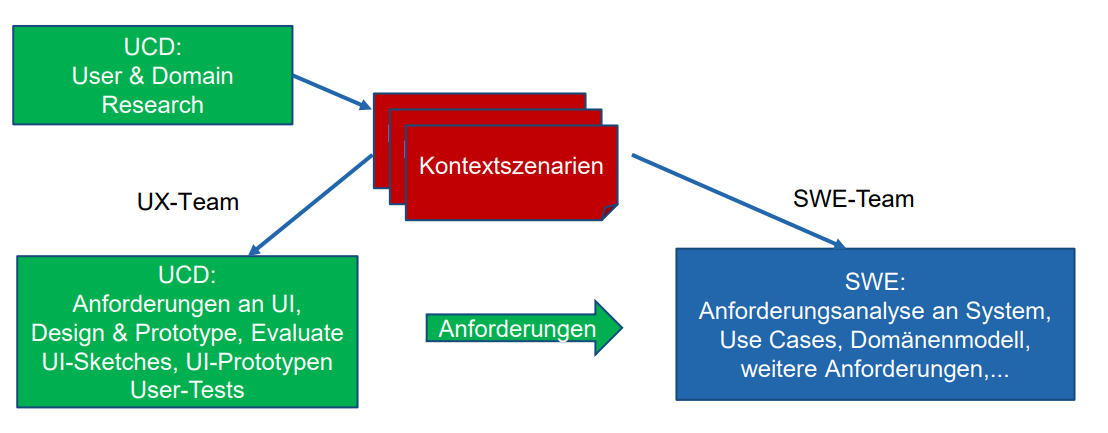
\includegraphics[width=\linewidth]{images/user_anforderungen.png}

\textbf{Charakteristiken:}
\begin{itemize}
    \item Können explizit oder implizit sein
    \item Sind fast nie im Vorneherein vollständig bekannt
    \item Müssen mit allen Stakeholdern erarbeitet werden
    \item Entwickeln sich während des Projekts
    \item Müssen verifizierbar und messbar sein
\end{itemize}

\textbf{Herkunft:}
\begin{itemize}
    \item Benutzer (Ziele, Bedürfnisse, Kontext)
    \item Weitere Stakeholder (Management, IT, etc.)
    \item Regulatorien, Gesetze, Normen
\end{itemize}
\end{definition}





\begin{concept}{Arten von Anforderungen}\\
\textbf{Funktionale Anforderungen:}
\begin{itemize}
    \item Beschreiben, WAS das System tun soll
    \item Werden in Use Cases dokumentiert
    \item Müssen konkret und testbar sein
\end{itemize}

\textbf{Nicht-funktionale Anforderungen (ISO 25010):}
\begin{itemize}
    \item Performance Efficiency
    \begin{itemize}
        \item Time Behaviour
        \item Resource Utilization
        \item Capacity
    \end{itemize}
    \item Compatibility
    \begin{itemize}
        \item Co-existence
        \item Interoperability
    \end{itemize}
    \item Usability (siehe oben)
    \item Reliability
    \begin{itemize}
        \item Maturity
        \item Availability
        \item Fault Tolerance
        \item Recoverability
    \end{itemize}
    \item Security
    \item Maintainability
    \item Portability
\end{itemize}

\textbf{Randbedingungen:}
\begin{itemize}
    \item Technische Einschränkungen
    \item Rechtliche Vorgaben
    \item Budgetäre Grenzen
    \item Zeitliche Limitationen
\end{itemize}
\end{concept}

\begin{KR}{Requirements Analysis}
    \begin{itemize}
        \item Benutzeranforderungen ableiten
        \item Kontextszenarien erstellen
        \item UI-Skizzen entwickeln
        \item Use Cases definieren
    \end{itemize}
    \vspace{2mm}

    \begin{minipage}[t]{0.45\linewidth}
    \textbf{Stakeholder identifizieren}
    \begin{itemize}
        \item Benutzer
        \item Auftraggeber
        \item Weitere Interessengruppen
    \end{itemize}
    
    \textbf{Anforderungsquellen \\ analysieren}
    \begin{itemize}
        \item Interviews und Workshops
        \item Existierende Dokumente
        \item Beobachtung der \\Arbeitsabläufe
    \end{itemize}
    \end{minipage}
    \begin{minipage}[t]{0.55\linewidth}    
    \textbf{Anforderungen dokumentieren}
    \begin{itemize}
        \item Funktionale Anforderungen \\ (Use Cases)
        \item Nicht-funktionale Anforderungen
        \item Randbedingungen
    \end{itemize}
    
    \textbf{Anforderungen validieren}
    \begin{itemize}
        \item Review mit Stakeholdern
        \item Priorisierung
        \item Machbarkeitsanalyse
    \end{itemize}
    \end{minipage}
\end{KR}

\begin{example2}{Anforderungsanalyse: Onlineshop}\\
\textbf{Ausgangssituation:}
Ein traditioneller Buchladen möchte einen Onlineshop entwickeln.

\textbf{Funktionale Anforderungen:}
\begin{itemize}
    \item Produktkatalog durchsuchen
    \item Warenkorb verwalten
    \item Bestellung aufgeben
    \item Kundenkonto verwalten
\end{itemize}

\textbf{Nicht-funktionale Anforderungen:}
\begin{itemize}
    \item Performance:
    \begin{itemize}
        \item Seitenaufbau < 2 Sekunden
        \item Suche < 1 Sekunde
    \end{itemize}
    \item Sicherheit:
    \begin{itemize}
        \item HTTPS-Verschlüsselung
        \item Zwei-Faktor-Authentifizierung
    \end{itemize}
    \item Usability:
    \begin{itemize}
        \item Responsive Design
        \item Max. 3 Klicks zur Bestellung
    \end{itemize}
\end{itemize}

\textbf{Randbedingungen:}
\begin{itemize}
    \item DSGVO-Konformität
    \item Integration mit bestehendem ERP
    \item Budget: 100.000 EUR
    \item Launch in 6 Monaten
\end{itemize}
\end{example2}

\columnbreak



\subsection{Use Cases}

\begin{definition}{Use Case (Anwendungsfall)}\\
Ein Use Case beschreibt eine konkrete Interaktion zwischen Akteur und System mit folgenden Eigenschaften:

\textbf{Grundprinzipien:}
\begin{itemize}
    \item Aus Sicht des Akteurs beschrieben
    \item Aktiv formuliert (Verb + Objekt)
    \item Konkreter Nutzen für Akteur
    \item Mehr als eine einzelne Interaktion
    \item Essentieller Stil (Logik statt Implementierung)
\end{itemize}

\textbf{Qualitätskriterien:}
\begin{itemize}
    \item Boss-Test: Sinnvolle Arbeitseinheit
    \item EBP-Test: Elementary Business Process
    \item Size-Test: Mehrere Interaktionen
\end{itemize}
\end{definition}

\begin{KR}{Use Case Erstellung}\\
Schritte zur Erstellung eines vollständigen Use Cases:
\begin{enumerate}
    \item \textbf{Identifikation:} siehe \textcolor{green}{\textbf{Use Case Identifikation}}
    \item \textbf{Dokumentation:}
    \begin{itemize}
        \item Brief/Casual für erste Analyse
        \item Fully-dressed für wichtige Use Cases
        \item Standardablauf und Erweiterungen
    \end{itemize}
    \item \textbf{Review:}
    \begin{itemize}
        \item Mit Stakeholdern abstimmen
        \item Auf Vollständigkeit prüfen
        \item Konsistenz sicherstellen
    \end{itemize}
\end{enumerate}
\end{KR}

\begin{theorem}{Use Case Identifikation}
\begin{enumerate}
    \item \textbf{Systemgrenzen definieren}
    \begin{itemize}
        \item Was gehört zum System?
        \item Was ist externe Umgebung?
    \end{itemize}
    \item \textbf{Akteure identifizieren}
    \item \textbf{Ziele ermitteln}
    \begin{itemize}
        \item Geschäftsziele
        \item Benutzerziele
        \item Systemziele
    \end{itemize}
\end{enumerate}
\end{theorem}

\begin{corollary}{Akteure in Use Cases}
\begin{itemize}
    \item \textbf{Primärakteur:} Initiiert den Use Case, erhält Hauptnutzen
    \item \textbf{Unterstützender Akteur:} Hilft bei der Durchführung
    \item \textbf{Offstage-Akteur:} Indirekt beteiligter Stakeholder
\end{itemize}
\end{corollary}

\begin{concept}{Use Case Beziehungen}\\
\textbf{Include-Beziehung:}
\begin{itemize}
    \item Ein UC schließt einen anderen UC ein
    \item Wiederverwendung von Funktionalität
    \item Obligatorische Beziehung
\end{itemize}

\textbf{Extend-Beziehung:}
\begin{itemize}
    \item Optionale Erweiterung eines UC
    \item Unter bestimmten Bedingungen
    \item Ursprünglicher UC bleibt unverändert
\end{itemize}

\textbf{Generalisierung:}
\begin{itemize}
    \item Spezialisierung von Akteuren/UCs
    \item Vererbung von Eigenschaften
    \item "ist-ein"-Beziehung
\end{itemize}
\end{concept}

\begin{concept}{Use Case Granularität}
\begin{enumerate}
    \item \textbf{Brief Use Case}
    \begin{itemize}
        \item Kurze Zusammenfassung
        \item Hauptablauf skizzieren
        \item Keine Details zu Varianten
    \end{itemize}
    \item \textbf{Casual Use Case}
    \begin{itemize}
        \item Mehrere Absätze
        \item Hauptvarianten beschreiben
        \item Informeller Stil
    \end{itemize}
    \item \textbf{Fully-dressed Use Case}
    \begin{itemize}
        \item Vollständige Struktur
        \item Alle Varianten
        \item Vor- und Nachbedingungen
        \item Garantien definieren
    \end{itemize}
\end{enumerate}
\end{concept}

\begin{KR}{Fully-dressed Use Case erstellen}

\begin{minipage}[t]{0.55\linewidth}
\textbf{1. Grundinformationen}
\begin{itemize}
    \item Aussagekräftiger Name (aktiv)
    \item Umfang (Scope)
    \item Ebene (Level)
    \item Primärakteur
\end{itemize}

\textbf{2. Stakeholder und Interessen}
\begin{itemize}
    \item Alle beteiligten Parteien
    \item Deren spezifische Interessen
\end{itemize}

\textbf{3. Vor- und Nachbedingungen}
\begin{itemize}
    \item Was muss vorher erfüllt sein?
    \item Was ist nachher garantiert?
\end{itemize}
\end{minipage}
\begin{minipage}[t]{0.45\linewidth}
\textbf{4. Standardablauf}
\begin{itemize}
    \item Nummerierte Schritte
    \item Akteur-System-Interaktion
    \item Klare Erfolgskriterien
\end{itemize}

\textbf{5. Erweiterungen}
\begin{itemize}
    \item Alternative Abläufe
    \item Fehlerszenarien
    \item Verzweigungen
\end{itemize}
\end{minipage}
\end{KR}

\begin{example2}{Brief Use Case}
\textbf{Verkauf abwickeln}

Kunde kommt mit Waren zur Kasse. Kassier erfasst alle Produkte. System berechnet Gesamtbetrag. Kassier nimmt Zahlung entgegen und gibt ggf. Wechselgeld. System druckt Beleg.
\end{example2}

%TODO: Add casual use case?

\begin{example2}{Casual Use Case}
\textbf{UC: Verkauf abwickeln}
Der Umfang des Use Cases ist das Kassensystem. Der Primärakteur ist der Kassier. 
Der Stakeholder ist der Kunde, der eine schnelle Abwicklung wünscht, und das Geschäft, das eine korrekte Abrechnung benötigt. 
Die Vorbedingung ist, dass die Kasse geöffnet ist.
\vspace{2mm}\\
Der Standardablauf ist wie folgt:
Kassier startet neuen Verkauf und System initialisiert neue Transaktion. Kassier erfasst Produkte und System zeigt Zwischensumme. 
Kassier schliesst Verkauf ab und System zeigt Gesamtbetrag. Kunde bezahlt und System druckt Beleg.
\end{example2}


\begin{example2}{Fully-dressed Use Case}
\textbf{UC: Verkauf abwickeln}
\begin{itemize}
    \item \textbf{Umfang:} Kassensystem
    \item \textbf{Primärakteur:} Kassier
    \item \textbf{Stakeholder:} Kunde (schnelle Abwicklung), Geschäft (korrekte Abrechnung)
    \item \textbf{Vorbedingung:} Kasse ist geöffnet
    \item \textbf{Standardablauf:}
    \begin{enumerate}
        \item Kassier startet neuen Verkauf
        \item System initialisiert neue Transaktion
        \item Kassier erfasst Produkte
        \item System zeigt Zwischensumme
        \item Kassier schliesst Verkauf ab
        \item System zeigt Gesamtbetrag
        \item Kunde bezahlt
        \item System druckt Beleg
    \end{enumerate}
\end{itemize}
\end{example2}

\begin{example2}{Fully-dressed Use Case}
\textbf{Aufgabe:} Erstellen Sie einen fully-dressed Use Case für ein Online-Bibliothekssystem. Fokus: "Buch ausleihen"

\textbf{Lösung:}
\begin{itemize}
    \item \textbf{Umfang:} Online-Bibliothekssystem
    \item \textbf{Primärakteur:} Bibliotheksnutzer
    \item \textbf{Stakeholder:} 
    \begin{itemize}
        \item Bibliotheksnutzer: Möchte Buch einfach ausleihen
        \item Bibliothek: Korrekte Erfassung der Ausleihe
    \end{itemize}
    \item \textbf{Vorbedingung:} Nutzer ist eingeloggt
    \item \textbf{Standardablauf:}
    \begin{enumerate}
        \item Nutzer sucht Buch
        \item System zeigt Verfügbarkeit
        \item Nutzer wählt Ausleihe
        \item System prüft Ausleihberechtigung
        \item System registriert Ausleihe
        \item System zeigt Bestätigung
    \end{enumerate}
    \item \textbf{Erweiterungen:}
    \begin{itemize}
        \item 2a: Buch nicht verfügbar
        \item 4a: Keine Ausleihberechtigung
    \end{itemize}
\end{itemize}
\end{example2}

\begin{example2}{Typische Prüfungsaufgabe: Use Case Analyse}\\
\textbf{Aufgabe:} Analysieren Sie den folgenden Use Case und identifizieren Sie mögliche Probleme:

\textbf{Use Case:} "Der Benutzer loggt sich ein und das System zeigt die Startseite. Er klickt auf den Button und die Daten werden in der Datenbank gespeichert."

\textbf{Probleme:}
\begin{itemize}
    \item Zu technisch/implementierungsnah
    \item Fehlende Akteurperspektive
    \item Unklarer Nutzen/Ziel
    \item Fehlende Alternativszenarien
    \item Keine Fehlerbehandlung
\end{itemize}

\textbf{Verbesserter Use Case:}
"Der Kunde möchte seine Bestelldaten speichern. Er bestätigt die Eingaben und erhält eine Bestätigung über die erfolgreiche Speicherung."
\end{example2}

\begin{example2}{Prüfungsaufgabe: Use Case Analyse}\\
\textbf{Aufgabe:} Analysieren Sie folgenden Use Case und verbessern Sie ihn.

\textbf{Ursprünglicher Use Case:}
"Der User loggt sich ein. Das System überprüft seine Credentials in der Datenbank. 
Bei erfolgreicher Validierung wird die Startseite angezeigt. Der User klickt auf 'Profil bearbeiten' 
und das System speichert die Änderungen in der Datenbank."

\textbf{Probleme:}
\begin{itemize}
    \item Technische Implementierungsdetails
    \item Fehlende Akteurperspektive
    \item Keine Alternativen/Fehlerbehandlung
    \item Unklarer Nutzen/Ziel
\end{itemize}

\textbf{Verbesserter Use Case:}
"Profilinformationen aktualisieren"
\begin{itemize}
    \item \textbf{Primärakteur:} Registrierter Benutzer
    \item \textbf{Vorbedingung:} Benutzer ist authentifiziert
    \item \textbf{Standardablauf:}
    \begin{enumerate}
        \item Benutzer wählt Profilbearbeitung
        \item System zeigt aktuelle Profildaten
        \item Benutzer ändert gewünschte Informationen
        \item System prüft Änderungen
        \item System bestätigt erfolgreiche Aktualisierung
    \end{enumerate}
    \item \textbf{Erweiterungen:}
    \begin{itemize}
        \item 4a: Ungültige Eingaben
        \item 4b: Verbindungsfehler
    \end{itemize}
\end{itemize}
\end{example2}



\columnbreak

\subsection{Use Case Diagrams}

\begin{definition}{Use Case Diagramm}\\
    Zeigt:
    \begin{itemize}
        \item Systemabgrenzung
        \item Akteure: Primärakteure initiieren UCs, unterstützende sind beteiligt
    \end{itemize}
    Liste der Anwendungsfälle:
    \begin{itemize}
        \item Process Sale
        \item Cash in
        \item Cash out
        \item Handle Returns
        \item Manage Users
    \end{itemize}
    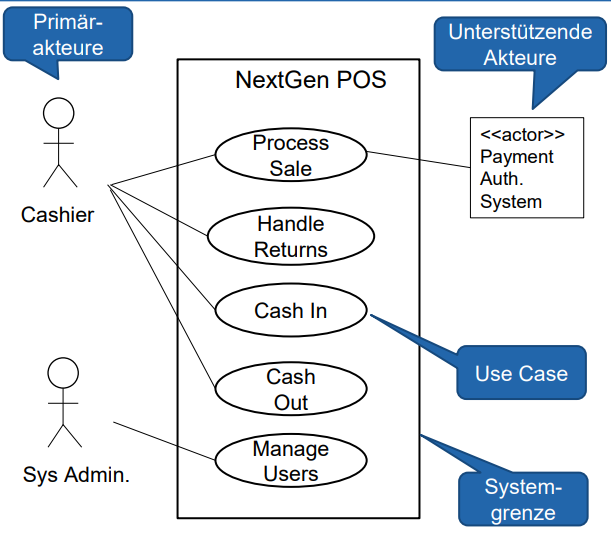
\includegraphics[width=\linewidth]{uc_diagram.png}
\end{definition}

\begin{concept}
    {Zusätzliche Beziehungen im UC-Diagramm}

    <<include>>
    \begin{itemize}
        \item Ein UC kann ein anderes UC inkludieren
        \item Wiederverwendung von Funktionalität
        \item Obligatorische Beziehung
        \item UC „Process Sale" inkludiert UC „Handle Cash Payment"
        \item UC „Process Sale" inkludiert UC „Handle TWINT Payment"
        \item Sie sind hier aber keine eigenständigen UCs (keine Verbindung zu Akteuren)
        \item Included UCs können auch selbständige UC sein.
    \end{itemize}
    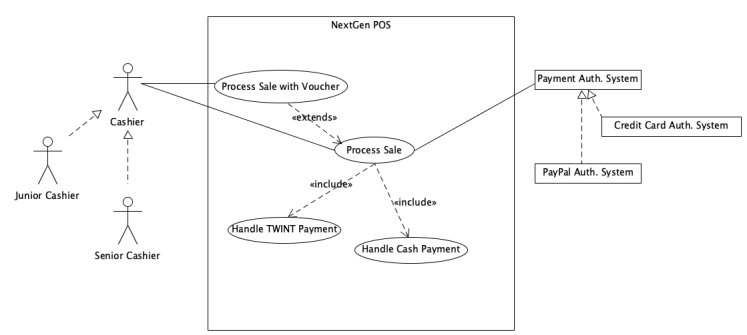
\includegraphics[width=\linewidth]{includebez.png}

    <<extends>>
    \begin{itemize}
        \item Eigenständiger UC, der eine Erweiterung eines anderen darstellt, und
        \item ursprünglicher UC nicht verändert werden soll
        \item Sonst besser als Erweiterung im UC-Text einfügen
        \item Akteur-Generalisierung
        \item Um Akteure zusammenzufassen
        \item Kann als „ist-ein"-Beziehung modelliert werden
    \end{itemize}
    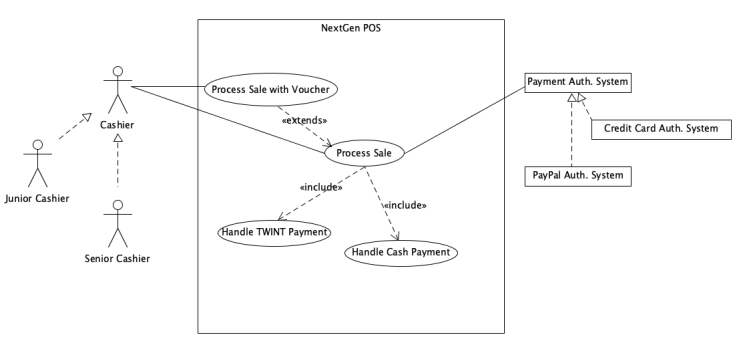
\includegraphics[width=\linewidth]{extendbez.png}
\end{concept}

\pagebreak

\subsection{System Sequence Diagrams}

\begin{definition}{Systemsequenzdiagramm (SSD)}\\
Formalisierte Darstellung der System-Interaktionen:

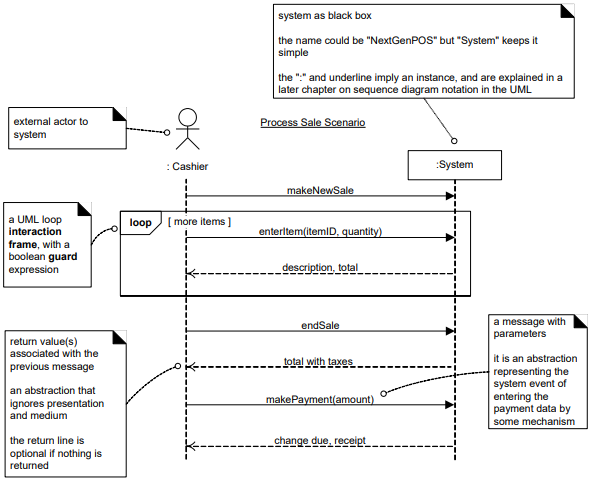
\includegraphics[width=\linewidth]{ssed.png}
\end{definition}

\begin{concept}{System Sequence Diagram}\\
Ein SSD visualisiert die Interaktion zwischen Akteur und System auf einer höheren Abstraktionsebene:

\textbf{Hauptmerkmale:}
\begin{itemize}
    \item Zeigt Input/Output-Events
    \item Identifiziert Systemoperationen
    \item Bildet Basis für API-Design
    \item Abstrahiert von UI-Details
\end{itemize}

\textbf{Notationselemente:}
\begin{itemize}
    \item Akteur und System als Lebenslinien
    \item Methodenaufrufe als durchgezogene Pfeile
    \item Rückgabewerte als gestrichelte Pfeile
    \item Parameter für benötigte Informationen
\end{itemize}
\end{concept}

\begin{KR}{System Sequence Diagram erstellen}\\
\textbf{1. Vorbereitung}
\begin{itemize}
    \item Use Case als Grundlage wählen
    \item Standardablauf identifizieren
    \item Akteur und System festlegen
\end{itemize}

\textbf{2. Methodenaufrufe definieren}
\begin{itemize}
    \item Aussagekräftige Namen wählen
    \item Notwendige Parameter bestimmen
    \item Rückgabewerte festlegen
\end{itemize}

\textbf{3. Zeitliche Abfolge}
\begin{itemize}
    \item Sequenz der Aufrufe modellieren
    \item Abhängigkeiten beachten
    \item Kontrollstrukturen einbauen (alt, loop, etc.)
\end{itemize}

\textbf{4. Externe Systeme}
\begin{itemize}
    \item Bei Bedarf weitere Akteure einbinden
    \item Schnittstellen definieren
    \item Kommunikationsfluss darstellen
\end{itemize}
\end{KR}

\begin{KR}{Systemoperationen definieren}\\
\textbf{Namenskonventionen:}
\begin{itemize}
    \item Verben für Aktionen
    \item Substantive für Entitäten
    \item Präzise, aber nicht technisch
\end{itemize}

\textbf{Parameter:}
\begin{itemize}
    \item Nur notwendige Information
    \item Domänenorientierte Typen
    \item Sinnvolle Standardwerte
\end{itemize}

\textbf{Rückgabewerte:}
\begin{itemize}
    \item Eindeutige Bestätigungen
    \item Relevante Geschäftsobjekte
    \item Fehlerindikationen
\end{itemize}

\textbf{Beispiele guter Operationen:}
\begin{lstlisting}[language=Java, style=base]
// Gut - klar und domaenenorientiert
createOrder(customer: CustomerId): OrderId
addOrderItem(orderId: OrderId, 
            product: ProductId, 
            quantity: int)

// Schlecht - zu technisch/implementierungsnah
insertIntoOrderTable(customerData: Map)
updateOrderItemList(items: ArrayList)
\end{lstlisting}
\end{KR}

\begin{KR}{Operation Contracts}\\
Ein Contract definiert die Vor- und Nachbedingungen einer Systemoperation:

\textbf{1. Struktur}
\begin{itemize}
    \item Name und Parameter
    \item Querverweis zum Use Case
    \item Vorbedingungen
    \item Nachbedingungen
\end{itemize}

\textbf{2. Vorbedingungen}
\begin{itemize}
    \item Systemzustand vor Aufruf
    \item Notwendige Initialisierungen
    \item Gültige Parameter
\end{itemize}

\textbf{3. Nachbedingungen}
\begin{itemize}
    \item Erstellte/gelöschte Instanzen
    \item Geänderte Attribute
    \item Neue/gelöschte Assoziationen
\end{itemize}
\end{KR}

\begin{remark}
    Wann Operation Contracts?

    - Nur wenn aus einem Anwendungsfall nicht klar wird, was die Systemoperation genau machen muss
    
    - Meist nur bei sehr komplizierten Operationen und/oder
    
    - Wenn Entwicklung der Systemoperation ausgelagert wird (anderes Team, externe Entwickler)
    
    - Erst gegen Ende des Meilensteins Lösungsarchitektur oder kurz vor Start des Designs der Systemoperation
\end{remark}

\begin{example2}{Contract für enterItem()}\\
\textbf{Operation:} enterItem(itemId: ItemID, quantity: int)

\textbf{Querverweis:} UC "Process Sale"

\textbf{Vorbedingungen:}
\begin{itemize}
    \item Verkauf ist gestartet
    \item ItemID existiert im System
\end{itemize}

\textbf{Nachbedingungen:}
\begin{itemize}
    \item SalesLineItem-Instanz wurde erstellt
    \item Verknüpfung mit aktueller Sale-Instanz
    \item quantity wurde gesetzt
    \item Verknüpfung mit ProductDescription
\end{itemize}
\end{example2}

\begin{example2}{SSD für Interaktion zwischen 2 Systemen}\\
    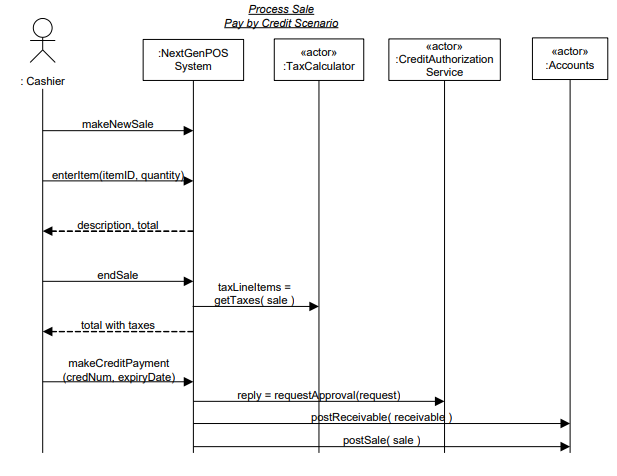
\includegraphics[width=\linewidth]{ssdzweisysteme.png}
\end{example2}


\begin{example2}{SSD Übungsaufgabe}\\
\textbf{Aufgabe:} Erstellen Sie ein Systemsequenzdiagramm für den Use Case 'Geld abheben' an einem Bankautomaten.

\textbf{Wichtige Aspekte:}
\begin{itemize}
    \item Kartenvalidierung
    \item PIN-Eingabe
    \item Betragseingabe
    \item Kontostandsprüfung
    \item Geldausgabe
    \item Belegdruck
\end{itemize}

\textbf{Essentielle Systemoperationen:}
\begin{itemize}
    \item validateCard(cardNumber)
    \item checkPIN(pin)
    \item withdrawMoney(amount)
    \item printReceipt()
\end{itemize}

\textbf{Sequenzdiagramm:} %TODO: add SSD graphic
\textcolor{pink}{\textbf{TO BE ADDED}}
\end{example2}


\begin{example2}{SSD: Online-Banking Überweisung}\\
\textbf{Use Case:} Überweisung durchführen

\textbf{Systemoperationen:}
\begin{lstlisting}[language=Java, style=base]
// Kontostand pruefen
checkBalance(): Money

// Ueberweisung initiieren
initiateTransfer(recipient: String, 
                iban: String, 
                amount: Money, 
                purpose: String): TransferId

// TAN anfordern
requestTAN(transferId: TransferId): void

// Ueberweisung bestaetigen
confirmTransfer(transferId: TransferId, 
               tan: String): Boolean
\end{lstlisting}

\textbf{Wichtige Aspekte:}
\begin{itemize}
    \item Validierung vor Ausführung
    \item Zweistufige Bestätigung
    \item Klare Rückmeldungen
    \item Fehlerbehandlung
\end{itemize}

\textbf{Sequenzdiagramm:} %TODO: add SSD graphic
\textcolor{pink}{\textbf{TO BE ADDED}}
\end{example2}


\begin{example2}{SSD: Typische Prüfungsaufgabe}\\
\textbf{Aufgabe:} Erstellen Sie ein SSD für den Use Case "Produkt bestellen" in einem Webshop.

\textbf{Analyse:}
\begin{itemize}
    \item Identifiziere Hauptaktionen:
    \begin{itemize}
        \item Warenkorb verwalten
        \item Bestellung aufgeben
        \item Zahlung durchführen
    \end{itemize}
    
    \item Definiere Systemoperationen:
    \begin{itemize}
        \item addToCart(productId, quantity)
        \item showCart(): CartContents
        \item checkout(shippingAddress, paymentMethod)
        \item confirmOrder(): OrderId
    \end{itemize}
    
    \item Berücksichtige Rückgabewerte:
    \begin{itemize}
        \item Bestätigungen
        \item Zwischensummen
        \item Fehlermeldungen
    \end{itemize}
\end{itemize}

\textbf{Sequenzdiagramm:} %TODO: add SSD graphic
\textcolor{pink}{\textbf{TO BE ADDED}}
\end{example2}


\begin{example2}{SSD: Integration mit externen Systemen}\\
\textbf{Use Case:} Kreditkartenzahlung durchführen

\textbf{Beteiligte Systeme:}
\begin{itemize}
    \item Verkaufssystem (SuD)
    \item Kreditkarten-Autorisierungssystem
    \item Buchhaltungssystem
\end{itemize}

\textbf{Systemoperationen:}
\begin{lstlisting}[language=Java, style=base]
// Request credit card approval
requestApproval(cardNum: String, 
               expiryDate: Date, 
               amount: Money): Boolean

// Post transaction to accounting
postTransaction(transactionData: TransactionData)
\end{lstlisting}

\textbf{Wichtige Aspekte:}
\begin{itemize}
    \item Asynchrone Kommunikation
    \item Fehlerbehandlung über mehrere Systeme
    \item Transaktionsmanagement
    \item Logging und Nachvollziehbarkeit
\end{itemize}

\textbf{Sequenzdiagramm:} %TODO: add SSD graphic
\textcolor{pink}{\textbf{TO BE ADDED}}
\end{example2}
	\raggedcolumns
	\pagebreak
	\input{02_domänenmodellierung.tex}
	\raggedcolumns
	\pagebreak
	\section{Softwarearchitektur und Design}

\begin{concept}{Überblick Softwareentwicklung}\\
Die Entwicklung von Software erfolgt in verschiedenen Ebenen:
\begin{itemize}
    \item Business Analyse (Domänenmodell, Requirements)
    \item Architektur (Logische Struktur)
    \item Entwicklung (Konkrete Umsetzung)
\end{itemize}
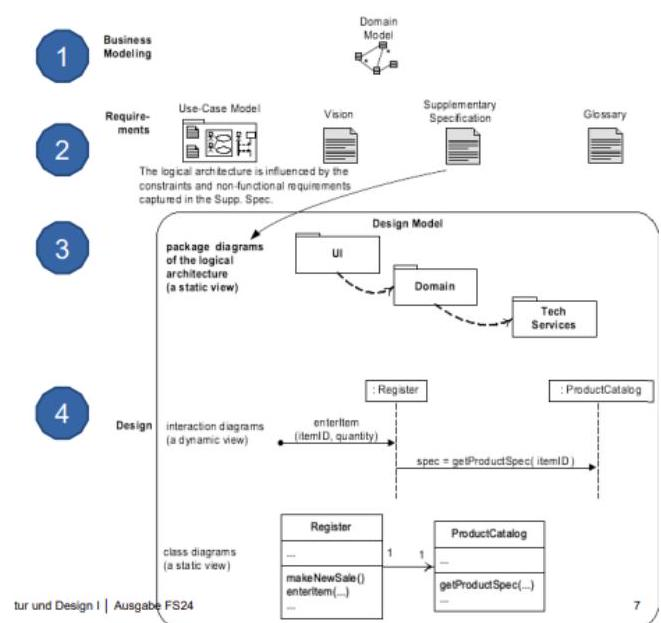
\includegraphics[width=0.9\linewidth]{images/2024_12_29_0d1d7b5551ea1b4b41bdg-07(2)}
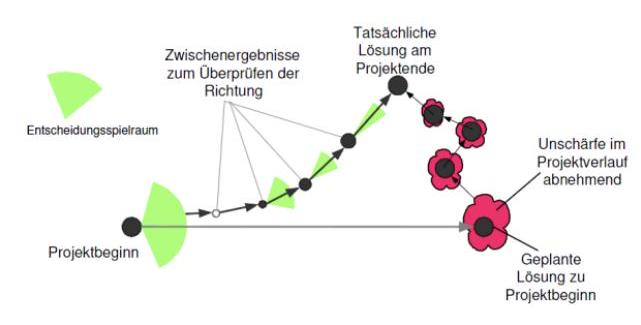
\includegraphics[width=0.9\linewidth]{images/2024_12_29_0d1d7b5551ea1b4b41bdg-08(1)}
\end{concept}

\begin{definition}{Softwarearchitektur}\\
Die Architektur definiert:
\begin{itemize}
    \item Grundlegende Strukturen und Komponenten
    \item Heutige und zukünftige Anforderungen
    \item Weiterentwicklungsmöglichkeiten
    \item Beziehungen zur Umgebung
\end{itemize}
\end{definition}

\begin{concept}{Architekturanalyse}\\
Die Analyse erfolgt iterativ mit den Anforderungen:
\begin{itemize}
    \item Analyse funktionaler und nicht-funktionaler Anforderungen
    \item Abstimmung mit Stakeholdern
    \item Kontinuierliche Weiterentwicklung
\end{itemize}
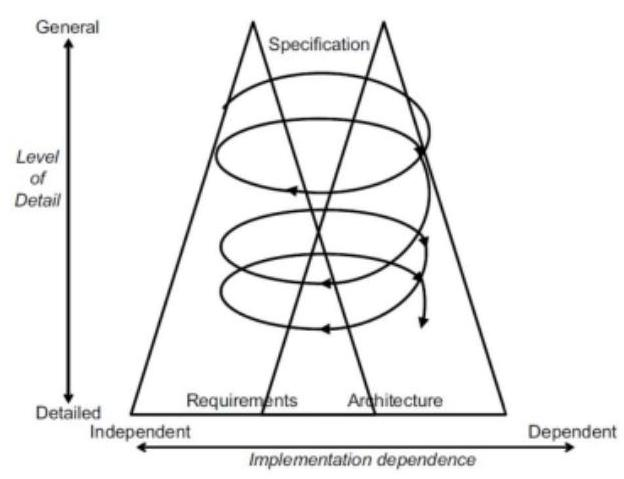
\includegraphics[width=0.9\linewidth]{images/2024_12_29_0d1d7b5551ea1b4b41bdg-08}
\end{concept}

\begin{theorem}{ISO 25010 vs FURPS+}\\
\textbf{ISO 25010:}
\begin{itemize}
    \item Hierarchische Struktur für nicht-funktionale Anforderungen
    \item Definierte Hauptcharakteristiken und Subcharakteristiken
    \item Messbare Metriken für jede Anforderung
    \item Präzise Formulierung und Verifikation
\end{itemize}

\textbf{FURPS+:}
\begin{itemize}
    \item Functionality (Funktionalität)
    \item Usability (Benutzbarkeit)
    \item Reliability (Zuverlässigkeit)
    \item Performance (Leistung)
    \item Supportability (Wartbarkeit)
    \item + (Implementation, Interface, Operations, Packaging, Legal)
\end{itemize}
\end{theorem}

\begin{concept}{Modulkonzept}\\
Ein Modul (Baustein, Komponente) wird bewertet nach:
\begin{itemize}
    \item \textbf{Kohäsion:} Innerer Zusammenhang
    \item \textbf{Kopplung:} Externe Abhängigkeiten
\end{itemize}

\textbf{Eigenschaften:}
\begin{itemize}
    \item Autarkes Teilsystem
    \item Minimale externe Schnittstellen
    \item Enthält alle benötigten Funktionen/Daten
    \item Verschiedene Formen: Paket, Library, Service
\end{itemize}
\end{concept}

\begin{KR}{Architekturentscheidungen treffen}
Systematischer Ansatz für Architekturentscheidungen:
\begin{enumerate}
    \item \textbf{Anforderungen analysieren}
    \begin{itemize}
        \item Funktionale Anforderungen gruppieren
        \item Nicht-funktionale Anforderungen priorisieren
        \item Randbedingungen identifizieren
    \end{itemize}
    
    \item \textbf{Einflussfaktoren bewerten}
    \begin{itemize}
        \item Technische Faktoren
        \item Organisatorische Faktoren
        \item Wirtschaftliche Faktoren
    \end{itemize}
    
    \item \textbf{Alternativen evaluieren}
    \begin{itemize}
        \item Vor- und Nachteile abwägen
        \item Proof of Concepts durchführen
        \item Risiken analysieren
    \end{itemize}
    
    \item \textbf{Entscheidung dokumentieren}
    \begin{itemize}
        \item Begründung festhalten
        \item Verworfene Alternativen dokumentieren
        \item Annahmen dokumentieren
    \end{itemize}
\end{enumerate}
\end{KR}

\begin{example2}{Typische Prüfungsaufgabe: Architekturanalyse}
\textbf{Aufgabenstellung:}
Analysieren Sie folgende Anforderungen und leiten Sie architektonische Konsequenzen ab:
\begin{itemize}
    \item System muss 24/7 verfügbar sein
    \item 10.000 gleichzeitige Benutzer
    \item Reaktionszeit unter 1 Sekunde
    \item Jährliche Wartungsfenster maximal 4 Stunden
\end{itemize}

\textbf{Lösung:}
\begin{itemize}
    \item \textbf{Architekturentscheidungen:}
    \begin{itemize}
        \item Verteilte Architektur für Hochverfügbarkeit
        \item Load Balancing für gleichzeitige Benutzer
        \item Caching-Strategien für Performanz
        \item Blue-Green Deployment für Wartung
    \end{itemize}
    
    \item \textbf{Begründungen:}
    \begin{itemize}
        \item Verteilung minimiert Single Points of Failure
        \item Load Balancer verteilt Last gleichmäßig
        \item Caching reduziert Datenbankzugriffe
        \item Blue-Green erlaubt Updates ohne Downtime
    \end{itemize}
\end{itemize}
\end{example2}

\begin{concept}{Architektursichten}\\
Das N+1 View Model beschreibt verschiedene Perspektiven:
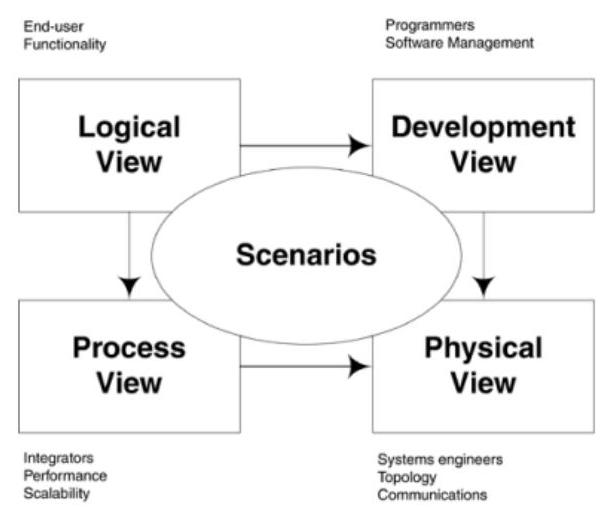
\includegraphics[width=0.9\linewidth]{images/2024_12_29_0d1d7b5551ea1b4b41bdg-09}

\textbf{UML-Paketdiagramm:}
\begin{itemize}
    \item Definition von Teilsystemen
    \item Gruppierung von Elementen
    \item Abhängigkeiten zwischen Paketen
\end{itemize}
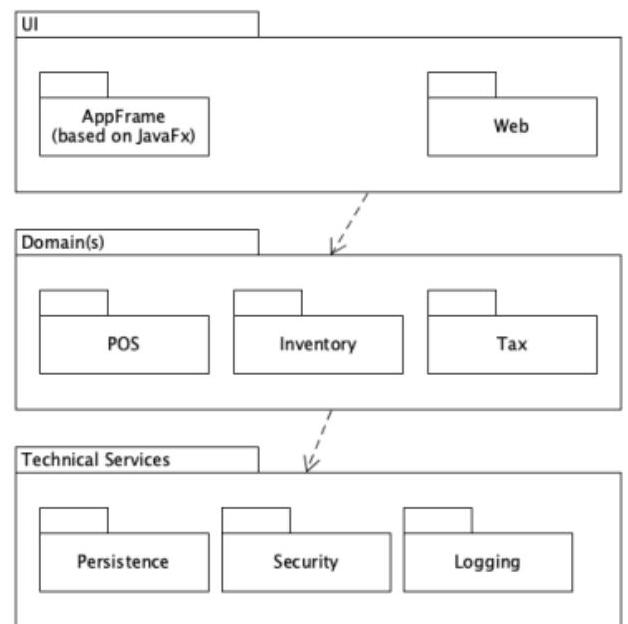
\includegraphics[width=0.9\linewidth]{images/2024_12_29_0d1d7b5551ea1b4b41bdg-09(1)}
\end{concept}

\begin{KR}{UML Diagrammauswahl}
Entscheidungshilfe für die Wahl des UML-Diagrammtyps:

\textbf{1. Strukturbeschreibung benötigt:}
\begin{itemize}
    \item Klassendiagramm für Typen und Beziehungen
    \item Paketdiagramm für Modularisierung
    \item Komponentendiagramm für Bausteinsicht
    \item Verteilungsdiagramm für Deployment
\end{itemize}

\textbf{2. Verhaltensbeschreibung benötigt:}
\begin{itemize}
    \item Sequenzdiagramm für Interaktionsabläufe
    \item Aktivitätsdiagramm für Workflows
    \item Zustandsdiagramm für Objektlebenszyklen
    \item Kommunikationsdiagramm für Objektkollaborationen
\end{itemize}

\textbf{3. Abstraktionsebene wählen:}
\begin{itemize}
    \item Analyse: Konzeptuelle Diagramme
    \item Design: Detaillierte Spezifikation
    \item Implementation: Codenahes Design
\end{itemize}
\end{KR}

\begin{example2}{GRASP Anwendung}
\textbf{Szenario:} Online-Shop Warenkorb-Funktionalität

\textbf{GRASP-Prinzipien angewandt:}
\begin{itemize}
    \item \textbf{Information Expert:}
    \begin{itemize}
        \item Warenkorb kennt seine Positionen
        \item Berechnet selbst Gesamtsumme
    \end{itemize}
    
    \item \textbf{Creator:}
    \begin{itemize}
        \item Warenkorb erstellt Warenkorbpositionen
        \item Bestellung erstellt aus Warenkorb
    \end{itemize}
    
    \item \textbf{Controller:}
    \begin{itemize}
        \item ShoppingController koordiniert UI und Domain
        \item Keine Geschäftslogik im Controller
    \end{itemize}
    
    \item \textbf{Low Coupling:}
    \begin{itemize}
        \item UI kennt nur Controller
        \item Domain unabhängig von UI
    \end{itemize}
\end{itemize}
\end{example2}

\begin{KR}{Architektur-Review durchführen}
\textbf{Vorgehen:}
\begin{enumerate}
    \item \textbf{Vorbereitung}
    \begin{itemize}
        \item Architektur-Dokumentation zusammenstellen
        \item Review-Team zusammenstellen
        \item Checklisten vorbereiten
    \end{itemize}
    
    \item \textbf{Durchführung}
    \begin{itemize}
        \item Architektur vorstellen
        \item Anforderungen prüfen
        \item Entscheidungen hinterfragen
        \item Risiken identifizieren
    \end{itemize}
    
    \item \textbf{Nachbereitung}
    \begin{itemize}
        \item Findings dokumentieren
        \item Maßnahmen definieren
        \item Follow-up planen
    \end{itemize}
\end{enumerate}

\textbf{Prüfkriterien:}
\begin{itemize}
    \item Anforderungserfüllung
    \item Technische Machbarkeit
    \item Zukunftssicherheit
    \item Best Practices
\end{itemize}
\end{KR}



\subsubsection{UML-Modellierung}

\begin{KR}{Statische vs. Dynamische Modelle}\\
\textbf{Statische Modelle (Struktur):}
\begin{itemize}
    \item UML-Klassendiagramm
    \item Fokus auf Pakete, Klassen, Attribute
    \item Keine Methodenimplementierung
\end{itemize}

\textbf{Dynamische Modelle (Verhalten):}
\begin{itemize}
    \item UML-Interaktionsdiagramme
    \item Fokus auf Logik und Verhalten
    \item Implementierung der Methoden
\end{itemize}
\end{KR}

\begin{definition}{UML-Diagrammtypen}\\
\textbf{1. Klassendiagramm:}
\begin{itemize}
    \item Klassen und aktive Klassen
    \item Attribute und Operationen
    \item Sichtbarkeiten und Beziehungen
    \item Interfaces und Realisierungen
\end{itemize}

\textbf{2. Sequenzdiagramm:}
\begin{itemize}
    \item Lebenslinien und Nachrichten
    \item Synchrone/Asynchrone Kommunikation
    \item Aktivierung und Deaktivierung
    \item Alternative Abläufe
\end{itemize}

\textbf{3. Zustandsdiagramm:}
\begin{itemize}
    \item Zustände und Übergänge
    \item Start- und Endzustände
    \item Composite States
    \item Historie und Parallelität
\end{itemize}

\textbf{4. Aktivitätsdiagramm:}
\begin{itemize}
    \item Aktionen und Aktivitäten
    \item Kontroll- und Datenflüsse
    \item Verzweigungen und Zusammenführungen
    \item Partitionen (Swimlanes)
\end{itemize}
\end{definition}

\begin{concept}{Responsibility Driven Design (RDD)}\\
Design basierend auf Verantwortlichkeiten:
\begin{itemize}
    \item Klassenentwurf nach Rollen
    \item Kollaborationsbeziehungen
    \item Implementierung durch Attribute/Methoden
    \item Anwendbar auf allen Ebenen
\end{itemize}
\end{concept}

\begin{theorem}{GRASP Prinzipien}\\
General Responsibility Assignment Software Patterns:
\begin{itemize}
    \item \textbf{Information Expert:} Verantwortung basierend auf Information
    \item \textbf{Creator:} Objekterstellung bei starker Beziehung
    \item \textbf{Controller:} Zentrale Steuerungslogik
    \item \textbf{Low Coupling:} Minimale Abhängigkeiten
    \item \textbf{High Cohesion:} Starker innerer Zusammenhang
    \item \textbf{Polymorphism:} Flexibilität durch Schnittstellen
    \item \textbf{Pure Fabrication:} Künstliche Klassen für besseres Design
    \item \textbf{Indirection:} Vermittler für Flexibilität
    \item \textbf{Protected Variations:} Kapselung von Änderungen
\end{itemize}
\end{theorem}

\begin{example2}{Architekturentwurf}
\textbf{Aufgabe:} Entwerfen Sie die grundlegende Architektur für ein Online-Banking-System.

\textbf{Lösung:}
\begin{itemize}
    \item \textbf{Anforderungsanalyse:}
    \begin{itemize}
        \item Sicherheit (ISO 25010)
        \item Performance (FURPS+)
        \item Skalierbarkeit
    \end{itemize}
    
    \item \textbf{Architekturentscheidungen:}
    \begin{itemize}
        \item Mehrschichtige Architektur
        \item Microservices für Skalierbarkeit
        \item Sicherheitsschicht
    \end{itemize}
    
    \item \textbf{Module:}
    \begin{itemize}
        \item Authentifizierung
        \item Transaktionen
        \item Kontoführung
    \end{itemize}
\end{itemize}
\end{example2}

\begin{KR}{Architekturentwurf}
\textbf{Schritte:}
\begin{enumerate}
    \item Anforderungen analysieren
    \item Architekturstil wählen
    \item Module identifizieren
    \item Schnittstellen definieren
    \item Mit Stakeholdern abstimmen
\end{enumerate}

\textbf{Qualitätskriterien:}
\begin{itemize}
    \item Änderbarkeit
    \item Wartbarkeit
    \item Erweiterbarkeit
    \item Testbarkeit
\end{itemize}
\end{KR}

\begin{example2}{Prüfungsaufgabe: UML-Modellierung}
\textbf{Aufgabe:} 
Modellieren Sie für ein Bibliothekssystem die Ausleihe eines Buches mit:
\begin{itemize}
    \item Klassendiagramm der beteiligten Klassen
    \item Sequenzdiagramm des Ausleihvorgangs
    \item Zustandsdiagramm für ein Buchexemplar
\end{itemize}

\textbf{Bewertungskriterien:}
\begin{itemize}
    \item Korrekte UML-Notation
    \item Vollständigkeit der Modellierung
    \item Konsistenz zwischen Diagrammen
    \item Angemessener Detaillierungsgrad
\end{itemize}
\end{example2}
	\raggedcolumns
	\pagebreak
	\section{Use Case Realization}

\begin{concept}{Use Case Realization}
Die Umsetzung von Use Cases erfolgt durch:
\begin{itemize}
    \item Detaillierte Szenarien aus den Use Cases
    \item Systemantworten müssen realisiert werden
    \item UI statt System im SSD
    \item Systemoperationen sind die zu implementierenden Elemente
\end{itemize}
\end{concept}

\subsection{Analyse-Artefakte}

\begin{concept}{Einfluss der Analyse-Artefakte}
\begin{itemize}
    \item \textbf{Use Cases:}
    \begin{itemize}
        \item Standardszenario
        \item Erweiterungen
        \item Definiert Systemoperationen
    \end{itemize}
    \item \textbf{Systemverträge:}
    \begin{itemize}
        \item Definieren Vorbedingungen
        \item Definieren Nachbedingungen
        \item Legen Invarianten fest
    \end{itemize}
    \item \textbf{Domänenmodell:}
    \begin{itemize}
        \item Inspiriert Softwareklassen
        \item Definiert Attribute
        \item Zeigt Beziehungen auf
    \end{itemize}
\end{itemize}
\end{concept}

\begin{KR}{Vorgehen bei der Use Case Realization}
\textbf{1. Vorbereitung}
\begin{itemize}
    \item Use Case auswählen und SSD ableiten
    \item Systemoperation identifizieren
    \item Operation Contract erstellen/prüfen
    \item Code/Dokumentation analysieren
    \item DCD überprüfen/aktualisieren
\end{itemize}

\textbf{2. Realisierung}
\begin{itemize}
    \item Controller Klasse bestimmen
    \item Zu verändernde Klassen festlegen
    \item Weg zu diesen Klassen festlegen
    \item Veränderungen implementieren
    \item Review durchführen
\end{itemize}
\end{KR}

\subsection{Design und Implementation}

\begin{concept}{UML im Design-Prozess}
UML dient als:
\begin{itemize}
    \item Zwischenschritt bei wenig Erfahrung
    \item Kompakter Ersatz für Programmiercode
    \item Kommunikationsmittel (auch für Nicht-Techniker)
\end{itemize}

\textbf{Arten der Modellierung:}
\begin{itemize}
    \item \textbf{Statische Modelle:} Klassenstruktur
    \item \textbf{Dynamische Modelle:} Verhalten
\end{itemize}
\end{concept}

\begin{KR}{Design to Code}
\textbf{Aus Design-Klassen-Diagramm (DCD):}
\begin{itemize}
    \item Klassen und deren Attribute
    \item Methoden und deren Signaturen
    \item Beziehungen zwischen Klassen
\end{itemize}

\textbf{Aus Interaktionsdiagrammen:}
\begin{itemize}
    \item Methodenaufrufe
    \item Parameter
    \item Sequenz der Aufrufe
\end{itemize}
\end{KR}

\subsection{GRASP Anwendung}

\begin{KR}{GRASP Patterns in der Realization}
\textbf{Die 5 wichtigsten Prinzipien:}
\begin{itemize}
    \item \textbf{Information Expert:}
    \begin{itemize}
        \item Verantwortlichkeit dort, wo Information liegt
        \item Basis für Methodenzuweisung
    \end{itemize}
    \item \textbf{Creator:}
    \begin{itemize}
        \item Regeln für Objekterzeugung
        \item Container erzeugt Inhalt
    \end{itemize}
    \item \textbf{Controller:}
    \begin{itemize}
        \item Erste Systemanlaufstelle
        \item Koordiniert Systemoperationen
    \end{itemize}
    \item \textbf{Low Coupling:}
    \begin{itemize}
        \item Minimale Abhängigkeiten
        \item Entscheidungshilfe bei Alternativen
    \end{itemize}
    \item \textbf{High Cohesion:}
    \begin{itemize}
        \item Fokussierte Verantwortlichkeiten
        \item Zusammengehörige Funktionalität
    \end{itemize}
\end{itemize}
\end{KR}

%todo: Add example of complete use case realization with all steps

\begin{KR}{Testing und Refactoring}
\textbf{1. Funktionale Prüfung}
\begin{itemize}
    \item Use Case Szenarien durchspielen
    \item Randfälle testen
    \item Fehlersituationen prüfen
\end{itemize}

\textbf{2. Strukturelle Prüfung}
\begin{itemize}
    \item Architekturkonformität
    \item GRASP-Prinzipien
    \item Clean Code Regeln
\end{itemize}

\textbf{3. Qualitätsprüfung}
\begin{itemize}
    \item Testabdeckung
    \item Wartbarkeit
    \item Performance
\end{itemize}
\end{KR}

%todo: Add testing examples and common refactoring scenarios
	\raggedcolumns
	\pagebreak
	\section{Design Patterns}

\begin{concept}{Grundlagen Design Patterns}
Bewährte Lösungsmuster für wiederkehrende Probleme:
\begin{itemize}
    \item Beschleunigen Entwicklung durch vorgefertigte Lösungen
    \item Verbessern Kommunikation im Team
    \item Bieten Balance zwischen Flexibilität und Komplexität
    \item \textbf{Wichtig:} Design Patterns sind kein Selbstzweck
\end{itemize}
\end{concept}

\begin{KR}{Pattern-Auswahl und Anwendung}
\begin{enumerate}
    \item Problem identifizieren
    \begin{itemize}
        \item Kernproblem isolieren
        \item Anforderungen analysieren
        \item Randbedingungen beachten
    \end{itemize}
    
    \item Patterns vergleichen
    \begin{itemize}
        \item Ähnliche Probleme suchen
        \item Lösungsansätze evaluieren
        \item Komplexität vs. Nutzen abwägen
    \end{itemize}
    
    \item Pattern anwenden
    \begin{itemize}
        \item An Kontext anpassen
        \item Minimale Implementation wählen
        \item Testbarkeit sicherstellen
    \end{itemize}
\end{enumerate}
\end{KR}

\subsection{Grundlegende Design Patterns}

\begin{example}{Adapter Pattern}
\begin{lstlisting}[language=Java]
// Externes Interface
interface LegacyPaymentProvider {
    boolean doPayment(double amount, String currency);
}

// Gewuenschtes Interface
interface PaymentService {
    PaymentResult processPayment(Money money);
}

// Adapter
class PaymentAdapter implements PaymentService {
    private LegacyPaymentProvider legacy;
    
    @Override
    public PaymentResult processPayment(Money money) {
        boolean success = legacy.doPayment(
            money.getAmount().doubleValue(),
            money.getCurrency().getCode()
        );
        return new PaymentResult(success);
    }
}
\end{lstlisting}
\end{example}

\begin{example}{Simple Factory}
\begin{lstlisting}[language=Java]
// Product Interface
interface Document {
    void open();
    void save();
}

// Concrete Products
class PDFDocument implements Document { /*...*/ }
class WordDocument implements Document { /*...*/ }

// Factory
class DocumentFactory {
    public Document createDocument(String type) {
        switch(type.toLowerCase()) {
            case "pdf": 
                return new PDFDocument();
            case "word": 
                return new WordDocument();
            default:
                throw new IllegalArgumentException(
                    "Unknown type: " + type);
        }
    }
}
\end{lstlisting}
\end{example}

\begin{example}{Singleton with Double-Checked Locking}
\begin{lstlisting}[language=Java]
public class DatabaseConnection {
    private static volatile DatabaseConnection instance;
    private final Connection connection;
    
    private DatabaseConnection() {
        // Private constructor
        connection = createConnection();
    }
    
    public static DatabaseConnection getInstance() {
        if (instance == null) {
            synchronized (DatabaseConnection.class) {
                if (instance == null) {
                    instance = new DatabaseConnection();
                }
            }
        }
        return instance;
    }
}
\end{lstlisting}
\end{example}

\begin{example}{Dependency Injection}
\begin{lstlisting}[language=Java]
// Service interfaces
interface MessageService {
    void sendMessage(String msg);
}

interface UserService {
    User findUser(String id);
}

// Service implementation with DI
class NotificationService {
    private final MessageService messageService;
    private final UserService userService;
    
    // Constructor injection
    public NotificationService(
            MessageService messageService,
            UserService userService) {
        this.messageService = messageService;
        this.userService = userService;
    }
    
    public void notifyUser(String userId, String message) {
        User user = userService.findUser(userId);
        messageService.sendMessage(
            String.format("To %s: %s", 
                user.getEmail(), message));
    }
}
\end{lstlisting}
\end{example}

\begin{example}{Chain of Responsibility}
\begin{lstlisting}[language=Java]
abstract class AuthenticationHandler {
    private AuthenticationHandler next;
    
    public void setNext(AuthenticationHandler next) {
        this.next = next;
    }
    
    public abstract boolean handle(String username, 
                                 String password);
    
    protected boolean handleNext(String username, 
                               String password) {
        if (next == null) {
            return false;
        }
        return next.handle(username, password);
    }
}

class DatabaseAuthHandler extends AuthenticationHandler {
    @Override
    public boolean handle(String username, 
                        String password) {
        // Check database
        boolean success = checkDatabase(username, 
                                      password);
        if (success) {
            return true;
        }
        return handleNext(username, password);
    }
}

class LDAPAuthHandler extends AuthenticationHandler {
    @Override
    public boolean handle(String username, 
                        String password) {
        // Check LDAP
        boolean success = checkLDAP(username, password);
        if (success) {
            return true;
        }
        return handleNext(username, password);
    }
}
\end{lstlisting}
\end{example}

[Continue with the rest of your original content, but with similar detailed examples for each pattern...]

\begin{KR}{Pattern Implementation Best Practices}
\begin{enumerate}
    \item \textbf{Interface Design}
    \begin{itemize}
        \item Klar und minimalistisch
        \item Erweiterbar gestalten
        \item Semantik dokumentieren
    \end{itemize}
    
    \item \textbf{Testbarkeit}
    \begin{itemize}
        \item Abhängigkeiten isolieren
        \item Mocking ermöglichen
        \item Verhalten verifizierbar
    \end{itemize}
    
    \item \textbf{Wartbarkeit}
    \begin{itemize}
        \item SOLID Prinzipien befolgen
        \item Dokumentation pflegen
        \item Komplexität minimieren
    \end{itemize}
\end{enumerate}
\end{KR}
	\raggedcolumns
	\pagebreak
	\section{Implementation, Refactoring und Testing}

\subsection{Design to Code}

\begin{concept}{Umsetzungsstrategien}
\textbf{Code-Driven Development:}
\begin{itemize}
    \item Direkte Implementierung der Klassen
    \item Nachträgliches Testing
\end{itemize}

\textbf{Test-Driven Development (TDD):}
\begin{itemize}
    \item Tests vor Implementation
    \item Red-Green-Refactor Zyklus
\end{itemize}

\textbf{Behavior-Driven Development (BDD):}
\begin{itemize}
    \item Testbeschreibung aus Anwendersicht
    \item Gherkin-Syntax für Szenarios
\end{itemize}
\end{concept}

\begin{KR}{Implementation Grundsätze}
\textbf{1. Code-Guidelines:}
\begin{itemize}
    \item Einheitliche Formatierung
    \item Klare Namenskonventionen
    \item Dokumentationsrichtlinien
\end{itemize}

\textbf{2. Fehlerbehandlung:}
\begin{itemize}
    \item Exceptions statt Fehlercodes
    \item Sinnvolle Error Messages
    \item Logging-Strategie
\end{itemize}

\textbf{3. Namensgebung:}
\begin{itemize}
    \item Aussagekräftige Namen
    \item Konsistente Begriffe
    \item Domain-Driven Naming
\end{itemize}
\end{KR}

\subsection{Refactoring}

\begin{definition}{Refactoring Grundlagen}
Strukturierte Verbesserung des Codes ohne Änderung des externen Verhaltens:
\begin{itemize}
    \item Kleine, kontrollierte Schritte
    \item Erhaltung der Funktionalität 
    \item Verbesserung der Codequalität und interner Struktur
    \item Ziel: Bessere Wartbarkeit und Erweiterbarkeit
\end{itemize}
\end{definition}

\begin{definition}{Code Smells}
Anzeichen für mögliche Probleme im Code:
\begin{itemize}
    \item Duplizierter Code
    \item Lange Methoden
    \item Klassen mit vielen Instanzvariablen
    \item Klassen mit sehr viel Code
    \item Auffällig ähnliche Unterklassen
    \item Keine Interfaces
    \item Hohe Kopplung zwischen Klassen
\end{itemize}
\end{definition}

\begin{KR}{Refactoring Patterns}
\textbf{1. Extract Method}
\begin{itemize}
    \item Code in eigene Methode auslagern
    \item Verbessert Lesbarkeit und Wiederverwendbarkeit
    \item Reduziert Duplikation
\end{itemize}

\textbf{2. Move Method/Field}
\begin{itemize}
    \item Methode/Feld in andere Klasse verschieben
    \item Verbessert Kohäsion
    \item Folgt Information Expert
\end{itemize}

\textbf{3. Extract Class}
\begin{itemize}
    \item Teil einer Klasse in neue Klasse auslagern
    \item Trennt Verantwortlichkeiten
    \item Erhöht Kohäsion
\end{itemize}

\textbf{4. Rename Method/Class/Variable}
\begin{itemize}
    \item Bessere Namen für besseres Verständnis
    \item Dokumentiert Zweck
    \item Erleichtert Wartung
\end{itemize}
\end{KR}

\subsection{Testing}

\begin{concept}{Teststufen}
\begin{itemize}
\item \textbf{Unit Tests:} 
\begin{itemize}
    \item Einzelne Komponenten
    \item Isolation durch Mocks/Stubs
    \item Schnelle Ausführung
\end{itemize}

\item \textbf{Integrationstests:} 
\begin{itemize} 
    \item Zusammenspiel mehrerer Komponenten
    \item Schnittstellen-Tests
    \item Externe Systeme
\end{itemize}

\item \textbf{Systemtests:} 
\begin{itemize}
    \item End-to-End Szenarien
    \item Nicht-funktionale Anforderungen
\end{itemize}

\item \textbf{Abnahmetests:} 
\begin{itemize}
    \item Gegen Kundenanforderungen
    \item User Acceptance Testing (UAT)
\end{itemize}
\end{itemize}
\end{concept}

\begin{KR}{Testdesign}
\textbf{1. Funktionaler Test (Black-Box)}
\begin{itemize}
    \item Test aus Benutzersicht
    \item Ohne Codekenntnis
    \item Fokus auf Input/Output
\end{itemize}

\textbf{2. Strukturbezogener Test (White-Box)}
\begin{itemize}
    \item Test mit Codekenntnis
    \item Code Coverage
    \item Pfadtests
\end{itemize}

\textbf{3. Änderungsbezogener Test}
\begin{itemize}
    \item Regressionstest
    \item Verifizierung von Änderungen
    \item Sicherstellung der Gesamtfunktionalität
\end{itemize}
\end{KR}

\begin{definition}{Testbegriffe}
\begin{itemize}
    \item \textbf{Testling/Testobjekt:} Das zu testende Element
    \item \textbf{Fehler:} Fehler des Entwicklers bei der Implementation
    \item \textbf{Fehlerwirkung/Bug:} Abweichung vom spezifizierten Verhalten
    \item \textbf{Testfall:} Spezifische Testkonfiguration mit Testdaten
    \item \textbf{Testtreiber:} Programm zur Testausführung
\end{itemize}
\end{definition}

%todo: Add examples for:
% - Refactoring before/after
% - Unit test with mocks
% - Integration test setup
% - Test case design examples
	\raggedcolumns
	\pagebreak
	[Previous content until initial definitions remains unchanged]

\begin{example}{Prüfungsaufgabe: Architekturstil-Analyse}
\textbf{Szenario:}
Ein Messaging-System soll entwickelt werden, das folgende Anforderungen erfüllt:
\begin{itemize}
    \item Hohe Skalierbarkeit
    \item Keine zentrale Komponente (Single Point of Failure)
    \item Direkter Nachrichtenaustausch zwischen Nutzern
    \item Offline-Fähigkeit
\end{itemize}

\textbf{Analysieren Sie die Architekturstile:}

\textbf{1. Client-Server}
\begin{itemize}
    \item \textbf{Vorteile:}
    \begin{itemize}
        \item Zentrale Verwaltung
        \item Einfache Konsistenzsicherung
    \end{itemize}
    \item \textbf{Nachteile:}
    \begin{itemize}
        \item Single Point of Failure
        \item Skalierungsprobleme
    \end{itemize}
\end{itemize}

\textbf{2. Peer-to-Peer}
\begin{itemize}
    \item \textbf{Vorteile:}
    \begin{itemize}
        \item Keine zentrale Komponente
        \item Direkte Kommunikation
        \item Gute Skalierbarkeit
    \end{itemize}
    \item \textbf{Nachteile:}
    \begin{itemize}
        \item Komplexe Konsistenzsicherung
        \item Schwierige Verwaltung
    \end{itemize}
\end{itemize}

\textbf{Empfehlung:} Peer-to-Peer mit hybriden Elementen
\end{example}

\begin{KR}{Verteilungsprobleme analysieren}
\textbf{1. Probleme identifizieren}
\begin{itemize}
    \item \textbf{Netzwerk:}
    \begin{itemize}
        \item Latenz
        \item Bandbreite
        \item Ausfälle
    \end{itemize}
    \item \textbf{Daten:}
    \begin{itemize}
        \item Konsistenz
        \item Replikation
        \item Synchronisation
    \end{itemize}
    \item \textbf{System:}
    \begin{itemize}
        \item Skalierung
        \item Verfügbarkeit
        \item Wartbarkeit
    \end{itemize}
\end{itemize}

\textbf{2. Lösungsstrategien entwickeln}
\begin{itemize}
    \item \textbf{Netzwerk:}
    \begin{itemize}
        \item Caching
        \item Compression
        \item Redundanz
    \end{itemize}
    \item \textbf{Daten:}
    \begin{itemize}
        \item Eventual Consistency
        \item Master-Slave Replikation
        \item Konfliktauflösung
    \end{itemize}
    \item \textbf{System:}
    \begin{itemize}
        \item Load Balancing
        \item Service Discovery
        \item Circuit Breaker
    \end{itemize}
\end{itemize}
\end{KR}

\begin{example}{Typische Prüfungsaufgabe: CAP-Theorem}
\textbf{Aufgabe:}
Analysieren Sie für ein verteiltes Datenbanksystem die Auswirkungen des CAP-Theorems.

\textbf{CAP-Theorem Komponenten:}
\begin{itemize}
    \item \textbf{Consistency:} Alle Knoten sehen dieselben Daten
    \item \textbf{Availability:} Jede Anfrage erhält eine Antwort
    \item \textbf{Partition Tolerance:} System funktioniert trotz Netzwerkausfällen
\end{itemize}

\textbf{Analyse der Trade-offs:}
\begin{itemize}
    \item \textbf{CA-System:}
    \begin{itemize}
        \item Hohe Konsistenz und Verfügbarkeit
        \item Keine Netzwerkpartitionierung möglich
        \item Beispiel: Traditionelle RDBMS
    \end{itemize}
    \item \textbf{CP-System:}
    \begin{itemize}
        \item Konsistenz und Partitionstoleranz
        \item Eingeschränkte Verfügbarkeit
        \item Beispiel: MongoDB
    \end{itemize}
    \item \textbf{AP-System:}
    \begin{itemize}
        \item Verfügbarkeit und Partitionstoleranz
        \item Eventual Consistency
        \item Beispiel: Cassandra
    \end{itemize}
\end{itemize}
\end{example}

\begin{KR}{Verteilte System-Design}
\textbf{1. Anforderungsanalyse}
\begin{itemize}
    \item \textbf{Funktional:}
    \begin{itemize}
        \item Kernfunktionalitäten
        \item Datenmodell
        \item Schnittstellen
    \end{itemize}
    \item \textbf{Nicht-funktional:}
    \begin{itemize}
        \item Skalierbarkeit
        \item Verfügbarkeit
        \item Latenz
    \end{itemize}
\end{itemize}

\textbf{2. Architekturentscheidungen}
\begin{itemize}
    \item \textbf{Kommunikation:}
    \begin{itemize}
        \item Synchron vs. Asynchron
        \item Push vs. Pull
        \item Protokollwahl
    \end{itemize}
    \item \textbf{Datenmanagement:}
    \begin{itemize}
        \item Sharding
        \item Replikation
        \item Caching
    \end{itemize}
\end{itemize}

\textbf{3. Implementierungsaspekte}
\begin{itemize}
    \item \textbf{Fehlerbehandlung:}
    \begin{itemize}
        \item Retry-Strategien
        \item Fallbacks
        \item Monitoring
    \end{itemize}
    \item \textbf{Sicherheit:}
    \begin{itemize}
        \item Authentifizierung
        \item Verschlüsselung
        \item Autorisierung
    \end{itemize}
\end{itemize}
\end{KR}

[Previous content about middleware and error sources remains]
	\raggedcolumns
	\pagebreak
	\subsection{Common Pitfalls und Best Practices}

\begin{concept}{Common Pitfalls in JPA Implementation}
\textbf{N+1 Problem:}
\begin{itemize}
    \item \textbf{Symptom:} Für jedes Objekt wird eine zusätzliche Query ausgeführt
    \item \textbf{Lösung:} Join Fetch oder Eager Loading strategisch einsetzen
\end{itemize}

\textbf{LazyInitializationException:}
\begin{itemize}
    \item \textbf{Symptom:} Zugriff auf lazy geladene Referenz außerhalb der Session
    \item \textbf{Lösung:} Transaktionen korrekt abgrenzen
\end{itemize}

\textbf{Bidirektionale Beziehungen:}
\begin{itemize}
    \item \textbf{Symptom:} Inkonsistente Objektzustände
    \item \textbf{Lösung:} Helper-Methoden für Beziehungspflege
\end{itemize}
\end{concept}

\begin{KR}{Best Practices für Persistenz}
\textbf{1. Architektur-Ebene}
\begin{itemize}
    \item Repository für Datenzugriff
    \item Service für Geschäftslogik
    \item DTO für Datentransfer
\end{itemize}

\textbf{2. Entity Design}
\begin{itemize}
    \item Immutable wenn möglich
    \item Bean Validation nutzen
    \item Geschäftsregeln in Entity-Klassen
\end{itemize}

\textbf{3. Performance}
\begin{itemize}
    \item Caching Strategien
    \item Batch Processing
    \item Query Optimierung
\end{itemize}
\end{KR}

\subsection{Parent-Child Beziehungen}

\begin{concept}{Parent-Child Mapping}
\textbf{Implementationsaspekte:}
\begin{itemize}
    \item Cascade-Typen definieren
    \item Bidirektionale Navigation
    \item Lazy Loading konfigurieren
    \item Orphan Removal festlegen
\end{itemize}

\textbf{JPA Annotationen:}
\begin{itemize}
    \item @OneToMany / @ManyToOne
    \item @JoinColumn
    \item mappedBy Parameter
    \item fetch = FetchType.LAZY/EAGER
\end{itemize}
\end{concept}

\subsection{Repository Pattern}

\begin{concept}{Spring Data Repository}
\textbf{Vorteile:}
\begin{itemize}
    \item Standardisierte CRUD-Operationen
    \item Query-Methoden aus Methodennamen
    \item Paginierung und Sortierung
    \item Einfache Integration mit Spring
\end{itemize}

\textbf{Repository Hierarchie:}
\begin{itemize}
    \item Repository (Marker Interface)
    \item CrudRepository (Basis CRUD)
    \item PagingAndSortingRepository
    \item JpaRepository (JPA-spezifisch)
\end{itemize}
\end{concept}

\begin{KR}{Repository Design}
\textbf{1. Interface Definition}
\begin{itemize}
    \item Domänenspezifische Methoden
    \item Query-Methoden
    \item Custom Implementations
\end{itemize}

\textbf{2. Query Methoden}
\begin{itemize}
    \item Methodennamen-Konventionen
    \item @Query Annotation
    \item Native Queries
\end{itemize}

\textbf{3. Transaktionshandling}
\begin{itemize}
    \item @Transactional Annotation
    \item Isolation Level
    \item Propagation Rules
\end{itemize}
\end{KR}

\subsection{Performance Optimierung}

\begin{KR}{Optimierungsstrategien}
\textbf{1. Fetch-Strategien}
\begin{itemize}
    \item Lazy Loading als Default
    \item Joins für häufig benötigte Daten
    \item EntityGraphs für komplexe Szenarien
\end{itemize}

\textbf{2. Caching}
\begin{itemize}
    \item First-Level Cache (Session)
    \item Second-Level Cache
    \item Query Cache
\end{itemize}

\textbf{3. Batch-Verarbeitung}
\begin{itemize}
    \item Batch Inserts/Updates
    \item JDBC Batch Size
    \item Pagination für große Datensätze
\end{itemize}
\end{KR}

%todo: Add examples for:
% - Handling parent-child relationships
% - Repository implementation with Spring Data
% - Performance optimization scenarios
% - Common pitfall solutions

\begin{concept}{Transaktionsmanagement}
\textbf{ACID-Eigenschaften:}
\begin{itemize}
    \item Atomicity (Atomarität)
    \item Consistency (Konsistenz)
    \item Isolation (Isolation)
    \item Durability (Dauerhaftigkeit)
\end{itemize}

\textbf{Isolation Levels:}
\begin{itemize}
    \item READ\_UNCOMMITTED
    \item READ\_COMMITTED
    \item REPEATABLE\_READ
    \item SERIALIZABLE
\end{itemize}
\end{concept}
	\raggedcolumns
	\pagebreak
	\section{Framework Design}

\begin{concept}{Framework Grundlagen}\\
Ein Framework ist ein Programmiergerüst mit folgenden Eigenschaften:
\begin{itemize}
    \item Bietet wiederverwendbare Funktionalität
    \item Definiert Erweiterungs- und Anpassungspunkte
    \item Verwendet Design Patterns
    \item Enthält keinen applikationsspezifischen Code
    \item Gibt Rahmen für anwendungsspezifischen Code vor
    \item Klassen arbeiten eng zusammen (vs. reine Bibliothek)
\end{itemize}
\end{concept}

\begin{definition}{Framework Entwicklung}\\
Die Entwicklung eines Frameworks erfordert:
\begin{itemize}
    \item Höhere Zuverlässigkeit als normale Software
    \item Tiefergehende Analyse der Erweiterungspunkte
    \item Hoher Architektur- und Designaufwand
    \item Sorgfältige Planung der Schnittstellen
\end{itemize}
\end{definition}

\begin{remark}{Kritische Betrachtung}\\
Herausforderungen beim Framework-Einsatz:
\begin{itemize}
    \item Frameworks tendieren zu wachsender Funktionalität
    \item Gefahr von inkonsistentem Design
    \item Funktionale Überschneidungen möglich
    \item Hoher Einarbeitungsaufwand
    \item Schwierige "Scheidung" nach Integration
    \item Trade-off zwischen Abhängigkeit und Nutzen
\end{itemize}
\end{remark}

\begin{KR}{Framework Design Principles}

\begin{minipage}[t]{0.5\textwidth}
\textbf{1. Abstraktionsebenen definieren}
\begin{itemize}
    \item \textbf{Core API:}
    \begin{itemize}
        \item Zentrale Interfaces
        \item Hauptfunktionalität
        \item Erweiterungspunkte
    \end{itemize}
    
    \item \textbf{Extensions:}
    \begin{itemize}
        \item Plugin-Mechanismen
        \item Callback-Interfaces
        \item Event-Systeme
    \end{itemize}
    
    \item \textbf{Implementierung:}
    \begin{itemize}
        \item Standard-Implementierungen
        \item Utility-Klassen
        \item Helper-Funktionen
    \end{itemize}
\end{itemize}
\end{minipage}
\begin{minipage}[t]{0.5\textwidth}
\textbf{2. Erweiterungsmechanismen}
\begin{itemize}
    \item \textbf{Interface-basiert:}
    \begin{itemize}
        \item Klare Verträge
        \item Lose Kopplung
        \item Einfache Erweiterung
    \end{itemize}
    
    \item \textbf{Annotations:}
    \begin{itemize}
        \item Deklarative Konfiguration
        \item Metadaten-getrieben
        \item Runtime-Processing
    \end{itemize}
    
    \item \textbf{Composition:}
    \begin{itemize}
        \item Plugin-System
        \item Service-Loader
        \item Dependency Injection
    \end{itemize}
\end{itemize}
\end{minipage}
\end{KR}

\begin{KR}{Analyse von Framework-Anforderungen}

\begin{minipage}[t]{0.5\textwidth}
\textbf{1. Fachliche Analyse}
\begin{itemize}
    \item \textbf{Core Features:}
    \begin{itemize}
        \item Zentrale Funktionalität
        \item Gemeinsame Abstraktionen
        \item Standardverhalten
    \end{itemize}
    \item \textbf{Variationspunkte:}
    \begin{itemize}
        \item Kundenspezifische\\ Anpassungen
        \item Optionale Features
        \item Erweiterungsmöglichkeiten
    \end{itemize}
\end{itemize}
\end{minipage}
\begin{minipage}[t]{0.5\textwidth}
\textbf{2. Technische Analyse}
\begin{itemize}
    \item \textbf{Architektur-Entscheidungen:}
    \begin{itemize}
        \item Erweiterungsmechanismen
        \item Integration in\\ bestehende Systeme
        \item Schnittstellen-Design
    \end{itemize}
    \item \textbf{Qualitätsanforderungen:}
    \begin{itemize}
        \item Performance
        \item Wartbarkeit
        \item Testbarkeit
    \end{itemize}
\end{itemize}
\end{minipage}
\end{KR}


\begin{example2}{Prüfungsaufgabe: Framework-Analyse}\\
\textbf{Szenario:}
Ein Framework für die Verarbeitung verschiedener Dokumentformate (PDF, DOC, TXT) 
soll entwickelt werden.

\textbf{Aufgabe:}
Analysieren Sie die Design-Entscheidungen.

\textbf{Lösung:}
\begin{itemize}
    \item \textbf{Erweiterungspunkte:}
    \begin{itemize}
        \item Dokumenttyp-Erkennung
        \item Parser für Formate
        \item Konvertierungslogik
    \end{itemize}
    
    \item \textbf{Design Patterns:}
    \begin{itemize}
        \item Factory für Parser-Erzeugung
        \item Strategy für Verarbeitungsalgorithmen
        \item Template Method für Konvertierung
    \end{itemize}
    
    \item \textbf{Schnittstellen:}
    \begin{itemize}
        \item DocumentParser Interface
        \item ConversionStrategy Interface
        \item DocumentMetadata Klasse
    \end{itemize}
\end{itemize}
\end{example2}



\subsection{Design Patterns in Frameworks}

\begin{concept}{Factory Method}\\
\textbf{Problem:} Flexible Objekterzeugung in wiederverwendbarer Klasse\\
\textbf{Lösung:}
\begin{itemize}
    \item Abstrakte Factory-Methode in Creator-Klasse
    \item Konkrete Subklassen überschreiben Methode
    \item Parallele Vererbungshierarchien
\end{itemize}
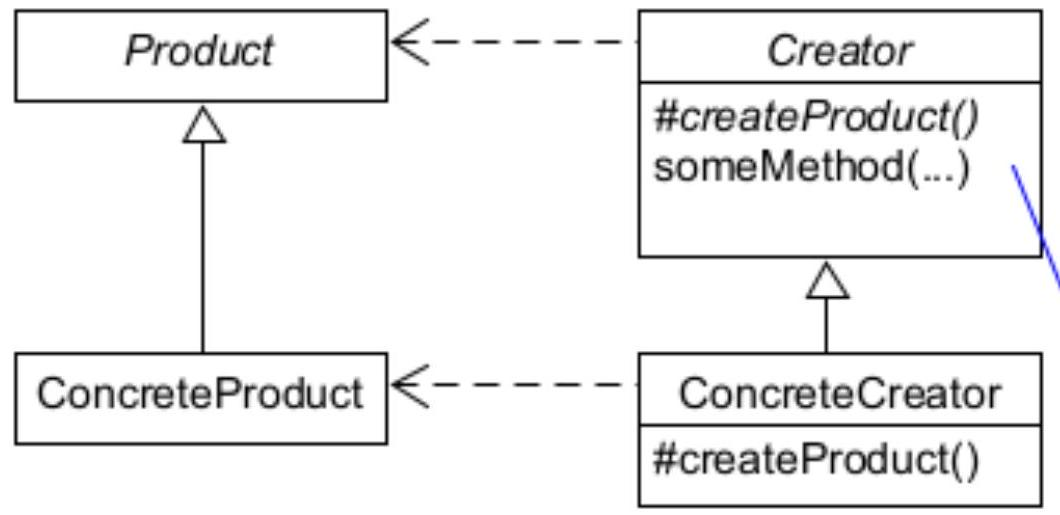
\includegraphics[width=0.6\linewidth]{images/2025_01_02_73d93f10fa91ab6123dcg-16}
\end{concept}

\begin{concept}{Abstract Factory}\\
\textbf{Problem:} Erzeugung verschiedener, zusammengehörender Objekte ohne Kenntnis konkreter Klassen\\
\textbf{Lösung:}
\begin{itemize}
    \item AbstractFactory-Interface definieren
    \item Pro Produkt eine create-Methode
    \item Konkrete Factories implementieren Interface
\end{itemize}
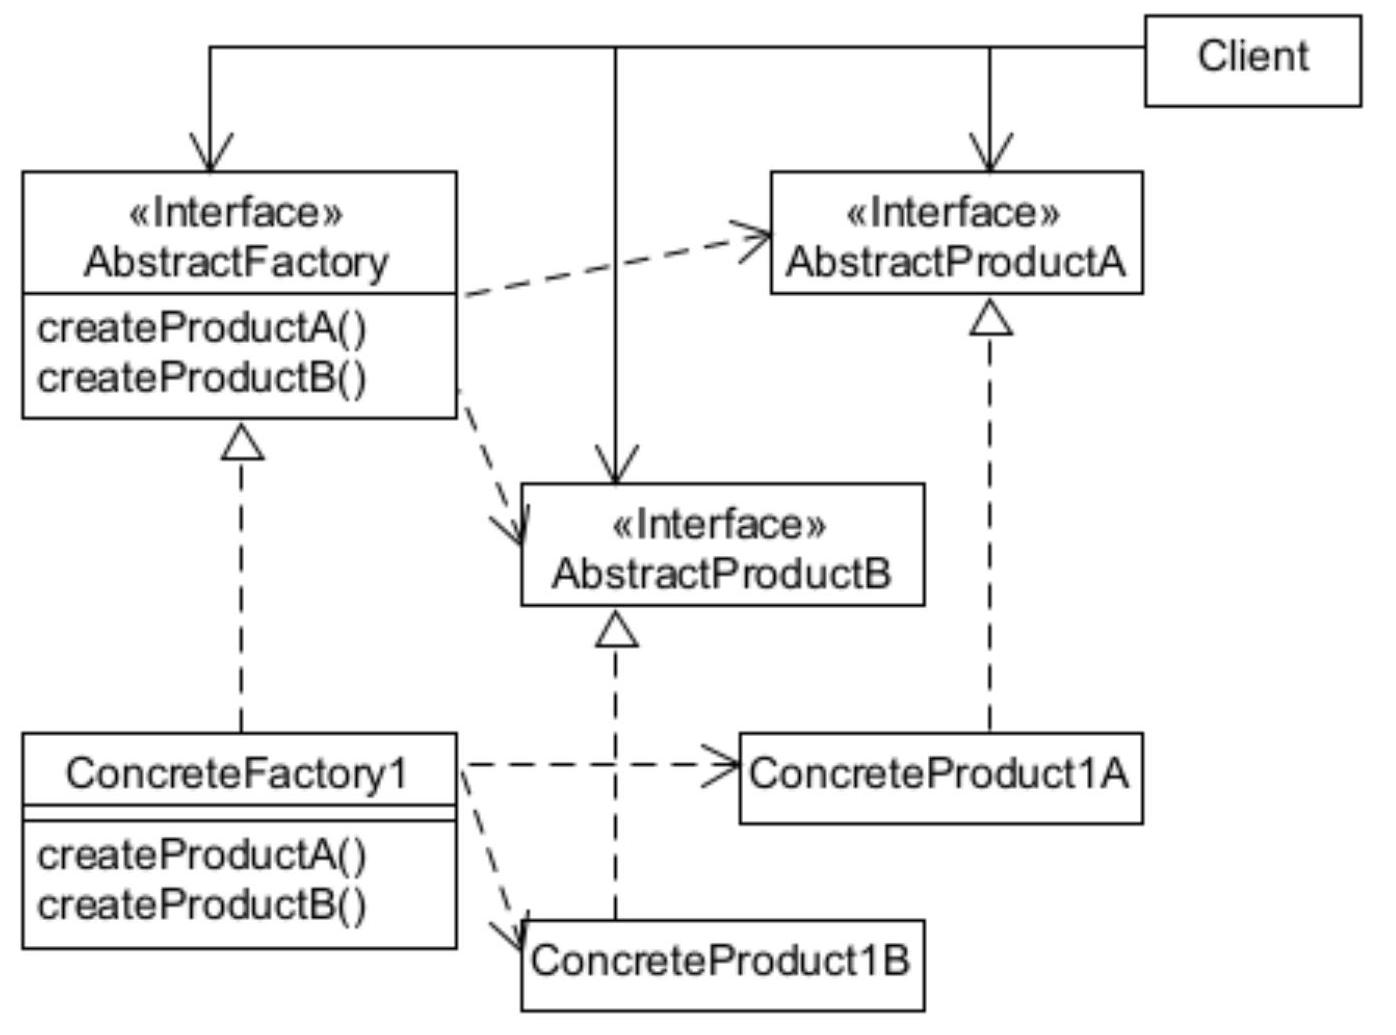
\includegraphics[width=0.8\linewidth]{images/2025_01_02_73d93f10fa91ab6123dcg-13}
\end{concept}


\begin{concept}{Command}\\
\textbf{Problem:} Aktionen für späteren Gebrauch speichern und verwalten\\
\textbf{Lösung:}
\begin{itemize}
    \item Command-Interface definieren
    \item Konkrete Commands implementieren
    \item Parameter für Ausführung speichern
    \item Optional: Undo-Funktionalität
\end{itemize}
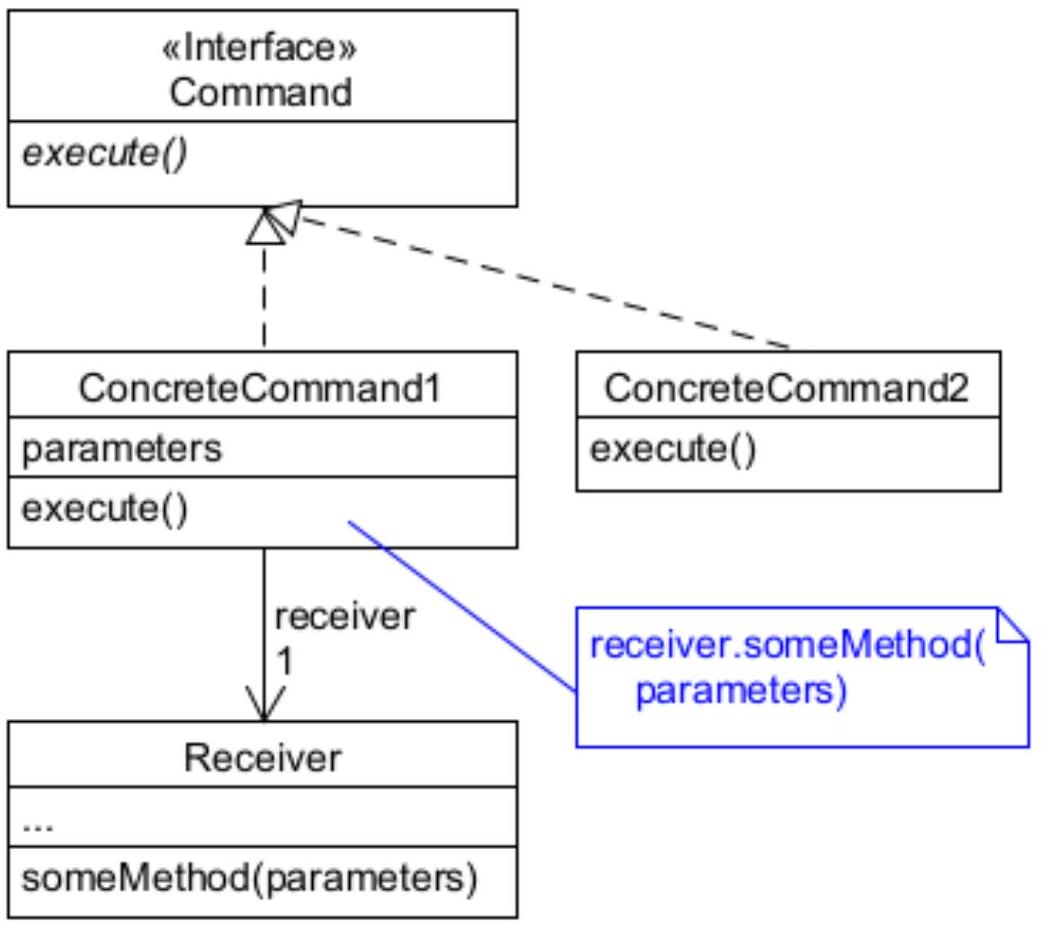
\includegraphics[width=0.7\linewidth]{images/2025_01_02_73d93f10fa91ab6123dcg-19}
\end{concept}


\begin{concept}{Template Method}\\
\textbf{Problem:} Algorithmus mit anpassbaren Teilschritten\\
\textbf{Lösung:}
\begin{itemize}
    \item Template Method in abstrakter Klasse
    \item Hook-Methoden für variable Teile
    \item Hollywood Principle: "Don't call us, we'll call you"
\end{itemize}
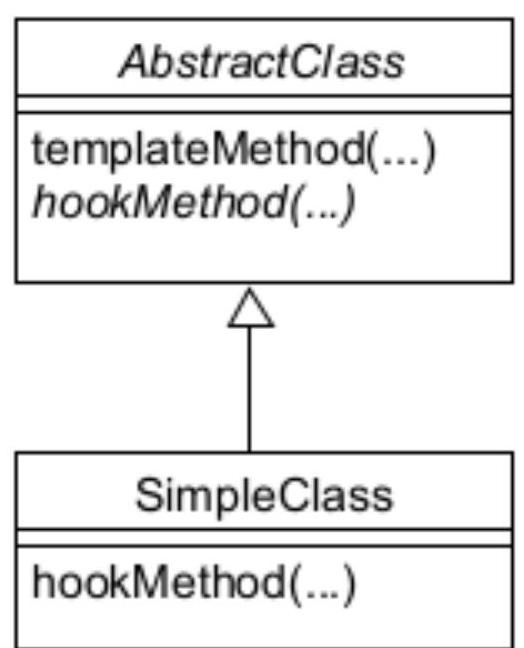
\includegraphics[width=0.3\linewidth]{images/2025_01_02_73d93f10fa91ab6123dcg-22}
\end{concept}

\begin{example2}{Framework Design Pattern Anwendung}\\
\textbf{Aufgabe:}
Implementieren Sie ein Plugin-System mit verschiedenen Design Patterns.

\textbf{Analyse der Pattern-Kombination:}
\begin{itemize}
    \item \textbf{Abstract Factory:}
    \begin{itemize}
        \item Plugin-Familie erzeugen
        \item Zusammengehörige Komponenten
        \item Austauschbare Implementierungen
    \end{itemize}
    
    \item \textbf{Template Method:}
    \begin{itemize}
        \item Plugin-Lifecycle definieren
        \item Standardablauf vorgeben
        \item Erweiterungspunkte bieten
    \end{itemize}
    
    \item \textbf{Command:}
    \begin{itemize}
        \item Plugin-Aktionen kapseln
        \item Asynchrone Ausführung
        \item Undo-Funktionalität
    \end{itemize}
\end{itemize}
\end{example2}


\subsection{Moderne Framework Mechanismen}

\begin{definition}{Annotation-basierte Konfiguration}\\
Moderne Frameworks nutzen Annotationen für:
\begin{itemize}
    \item Dependency Injection
    \item Konfiguration
    \item Interface-Implementation
    \item Funktionalitätserweiterung
\end{itemize}
\end{definition}

\begin{concept}{Annotations als Steuerungsmechanismus}\\
\textbf{Vorteile von Annotations:}
\begin{itemize}
    \item Keine harte Abhängigkeit zum Framework\\ (geringere Kopplung zur API)
    \item Annotation wird stillschweigend entfernt wenn nicht gefunden
    \item Geeignet für Domänenlogik ohne technische Abhängigkeiten
    \item Deklarativer Programmierstil
    \item Reduzierung von Boilerplate-Code
\end{itemize}

\textbf{Nachteil von Annotations:} Kann zu längeren Startzeiten führen
\end{concept}

\begin{theorem}{Auswertung von Annotations:}
\begin{itemize}
    \item \textbf{Startzeitpunkt:}
    \begin{itemize}
        \item Framework wird mit Anwendung gestartet
        \item Sucht Anwendungsklassen auf dem Klassenpfad
        \item Untersucht Annotationen
    \end{itemize}
    \item \textbf{Mögliche Framework-Aktionen:}
    \begin{itemize}
        \item Dependency Injection in Anwendungsobjekte
        \item Automatische Interface-Implementierung
        \item Funktionalität zu Klassen hinzufügen
    \end{itemize}
\end{itemize}
\end{theorem}

\begin{concept}{Aspekt-orientierte Programmierung in Frameworks}\\
\textbf{Querschnittliche Belange (Cross-Cutting Concerns):}
\begin{itemize}
    \item Logging
    \item Sicherheit
    \item Transaktionsmanagement
    \item Performance Monitoring
\end{itemize}

\textbf{Implementation mit Annotations:}
\begin{lstlisting}[language=Java, style=basesmol]
@Aspect
public class LoggingAspect {
    @Around("@annotation(Logged)")
    public Object logMethod(
            ProceedingJoinPoint joinPoint) 
            throws Throwable {
        
        String methodName = 
            joinPoint.getSignature().getName();
        Logger.info("Entering " + methodName);
        
        try {
            Object result = joinPoint.proceed();
            Logger.info("Exiting " + methodName);
            return result;
        } catch (Exception e) {
            Logger.error("Error in " + methodName, e);
            throw e;
        }
    }
}
// Usage in Framework Client Code
@Logged
public void businessMethod() {
    // Method implementation
}
\end{lstlisting}
\end{concept}



\begin{KR}{Java Mechanismen für Framework-Implementation}

    \begin{minipage}[t]{0.55\textwidth}
\textbf{1. Zeitpunkte für Code-Generierung}
\begin{itemize}
    \item \textbf{Compile-Zeit:}
    \begin{itemize}
        \item AnnotationProcessor
        \item Quellcode oder Bytecode generieren
    \end{itemize}
    \item \textbf{Laufzeit:}
    \begin{itemize}
        \item Beim Laden der Klassen
        \item Framework-Classloader
        \item Bytecode-Modifikation
    \end{itemize}
\end{itemize}
\end{minipage}
\begin{minipage}[t]{0.45\textwidth}
\textbf{2. Implementierungstechniken}
\begin{itemize}
    \item \textbf{Code Generation:}
    \begin{itemize}
        \item Quellcode hinzufügen
        \item Bytecode modifizieren
    \end{itemize}
    \item \textbf{Proxy Generation:}
    \begin{itemize}
        \item java.lang.reflect.Proxy
        \item Interface-Implementation
    \end{itemize}
\end{itemize}
\end{minipage}
\end{KR}

\begin{formula}{Framework Evaluation}

    \begin{minipage}[t]{0.5\textwidth}
\textbf{1. Qualitätskriterien}
\begin{itemize}
    \item \textbf{Usability:}
    \begin{itemize}
        \item Intuitive API
        \item Gute Dokumentation
        \item Beispiele/Templates
    \end{itemize}
    
    \item \textbf{Flexibilität:}
    \begin{itemize}
        \item Erweiterbarkeit
        \item Konfigurierbarkeit
        \item Modularität
    \end{itemize}
    
    \item \textbf{Wartbarkeit:}
    \begin{itemize}
        \item Klare Struktur
        \item Testbarkeit
        \item Versionierung
    \end{itemize}
\end{itemize}
\end{minipage}
\begin{minipage}[t]{0.5\textwidth}
\textbf{2. Risikobewertung}
\begin{itemize}
    \item \textbf{Technisch:}
    \begin{itemize}
        \item Kompatibilität
        \item Performance
        \item Skalierbarkeit
    \end{itemize}
    
    \item \textbf{Organisatorisch:}
    \begin{itemize}
        \item Learning Curve
        \item Support/Community
        \item Zukunftssicherheit
    \end{itemize}
\end{itemize}
\end{minipage}
\end{formula}

\begin{example2}{Prüfungsaufgabe: Framework Design Entscheidungen}\\
\textbf{Szenario:}
Sie sollen für eine Firma ein Framework zum Verarbeiten von Datenexporten entwickeln.
Die Firma arbeitet mit verschiedenen Datenformaten (CSV, Excel, XML) und möchte das 
Framework später einfach um weitere Formate erweitern können.

\textbf{Aufgabenstellung:}
\begin{enumerate}
    \item Identifizieren Sie die Variationspunkte
    \item Wählen Sie geeignete Design Patterns
    \item Skizzieren Sie die Framework-Architektur
\end{enumerate}

\textbf{Musterlösung:}
\begin{itemize}
    \item \textbf{Variationspunkte:}
    \begin{itemize}
        \item Format-Erkennung
        \item Datei-Parser
        \item Daten-Transformation
        \item Export-Ziele
    \end{itemize}
    
    \item \textbf{Design Patterns:}
    \begin{itemize}
        \item Abstract Factory für Parser-Erzeugung
        \item Strategy für unterschiedliche Parse-Algorithmen
        \item Template Method für generellen Export-Workflow
        \item Chain of Responsibility für Format-Erkennung
    \end{itemize}
    
    \item \textbf{Framework-Architektur:}
    \begin{itemize}
        \item Core API mit Interfaces
        \item Plugin-System für neue Formate
        \item Event-System für Export-Status
        \item Konfigurationsschicht
    \end{itemize}
\end{itemize}
\end{example2}

\columnbreak

\begin{example2}{Framework Design Pattern Kombination}\\
\textbf{Aufgabe:} 
Analysieren Sie die Kombination verschiedener Design Patterns in einem Framework.

\textbf{Muster-Framework:}
Event-Processing Framework mit folgenden Patterns:

\textbf{1. Template Method}
\begin{itemize}
    \item Definiert Workflow für Event-Verarbeitung
    \item Hook-Methoden für:
    \begin{itemize}
        \item Event-Validierung
        \item Event-Transformation
        \item Event-Persistierung
    \end{itemize}
\end{itemize}

\textbf{2. Chain of Responsibility}
\begin{itemize}
    \item Event-Handler-Kette
    \item Flexible Verarbeitungsreihenfolge
    \item Dynamische Handler-Registration
\end{itemize}

\textbf{3. Command}
\begin{itemize}
    \item Kapselung von Event-Handling-Logik
    \item Queuing von Events
    \item Undo/Redo Funktionalität
\end{itemize}

\textbf{4. Observer}
\begin{itemize}
    \item Benachrichtigung über Event-Status
    \item Lose Kopplung zwischen Komponenten
    \item Flexible Registration von Listeners
\end{itemize}

\textbf{Pattern-Interaktion:}
\begin{itemize}
    \item Template Method definiert Grundstruktur
    \item Chain of Responsibility organisiert Handler
    \item Command kapselt konkrete Aktionen
    \item Observer informiert über Ergebnisse
\end{itemize}
\end{example2}

\begin{example2}{Prüfungsaufgabe: Framework Testing}\\
\textbf{Szenario:}
Ein Framework soll gründlich getestet werden. Entwickeln Sie eine Teststrategie.

\textbf{Testebenen:}
\begin{itemize}
    \item \textbf{Unit Tests:}
    \begin{itemize}
        \item Einzelne Komponenten
        \item Mock-Objekte für Dependencies
        \item Edge Cases
    \end{itemize}
    
    \item \textbf{Integration Tests:}
    \begin{itemize}
        \item Zusammenspiel der Komponenten
        \item Plugin-Mechanismen
        \item Event-Handling
    \end{itemize}
    
    \item \textbf{System Tests:}
    \begin{itemize}
        \item End-to-End Szenarien
        \item Performance Tests 
        \item Load Tests
    \end{itemize}
\end{itemize}

\textbf{Besondere Aspekte:}
\begin{itemize}
    \item Extension Points testen
    \item Verschiedene Konfigurationen
    \item Backward Compatibility
    \item Error Handling
\end{itemize}
\end{example2}

\columnbreak

\begin{KR}{Framework-Extensions entwickeln}\\
\textbf{1. Extension Points identifizieren}
\begin{itemize}
    \item Core-Funktionalität analysieren
    \item Variationspunkte bestimmen
    \item Interface-Hierarchie planen
\end{itemize}

\textbf{2. Extension Mechanismen}
\begin{itemize}
    \item \textbf{Interface-basiert:}
    \begin{lstlisting}[language=Java, style=basesmol]
public interface Plugin {
    void initialize();
    void shutdown();
    String getName();
}
    \end{lstlisting}
    
    \item \textbf{Annotation-basiert:}
    \begin{lstlisting}[language=Java, style=basesmol]
@Extension
public class CustomPlugin {
    @Initialize
    public void setup() { ... }
    
    @Shutdown
    public void cleanup() { ... }
}
    \end{lstlisting}
\end{itemize}

\textbf{3. Discovery Mechanism}
\begin{lstlisting}[language=Java, style=basesmol]
public class ExtensionLoader {
    public List<Plugin> loadPlugins() {
        ServiceLoader<Plugin> loader = 
            ServiceLoader.load(Plugin.class);
        return StreamSupport
            .stream(loader.spliterator(), false)
            .collect(Collectors.toList());
    }
}
\end{lstlisting}
\end{KR}

\begin{example2}{Prüfungsaufgabe: Framework Evolution}\\
\textbf{Ausgangslage:}
Ein bestehendes Framework soll um neue Funktionalität erweitert werden, ohne bestehende 
Clients zu beeinträchtigen.

\textbf{Analyse der Optionen:}
\begin{itemize}
    \item \textbf{Annotation-basierte Erweiterung:}
    \begin{itemize}
        \item Vorteile:
        \begin{itemize}
            \item Keine Änderung bestehender Interfaces
            \item Optionale Funktionalität
            \item Deklarativer Ansatz
        \end{itemize}
        \item Nachteile:
        \begin{itemize}
            \item Komplexere Verarbeitung
            \item Mögliche Performance-Einbußen
            \item Schwieriger zu debuggen
        \end{itemize}
    \end{itemize}
    
    \item \textbf{Interface-basierte Erweiterung:}
    \begin{itemize}
        \item Vorteile:
        \begin{itemize}
            \item Klare Kontrakte
            \item Compile-time Checks
            \item Einfache Dokumentation
        \end{itemize}
        \item Nachteile:
        \begin{itemize}
            \item Änderungen an Interfaces nötig
            \item Adapter für alte Clients
            \item Höherer Implementierungsaufwand
        \end{itemize}
    \end{itemize}
\end{itemize}
\end{example2}

\columnbreak

\begin{KR}{Framework Integration}
\begin{enumerate}
    \item \textbf{Convention over Configuration}
    \begin{itemize}
        \item Namenskonventionen einhalten
        \item Standard-Verhalten nutzen
        \item Nur Ausnahmen konfigurieren
    \end{itemize}
    
    \item \textbf{Dependency Injection}
    \begin{itemize}
        \item Abhängigkeiten deklarieren
        \item Framework übernimmt Injection
        \item Constructor- oder Setter-Injection
    \end{itemize}
    
    \item \textbf{Interface-basierte Entwicklung}
    \begin{itemize}
        \item Interfaces definieren
        \item Framework generiert Implementation
        \item Methodennamen als Spezifikation
    \end{itemize}
\end{enumerate}
\end{KR}




\begin{example2}{Framework Integration Case Study}\\
\textbf{Szenario:}
Integration eines Logging-Frameworks in eine bestehende Anwendung

\textbf{Anforderungen:}
\begin{itemize}
    \item Minimale Änderungen am bestehenden Code
    \item Konfigurierbare Log-Level
    \item Verschiedene Log-Ausgaben (Konsole, File, DB)
    \item Performance-Monitoring
\end{itemize}

\textbf{Lösung mit Framework Patterns:}
\begin{lstlisting}[language=Java, style=basesmol]
// Logger Interface
public interface Logger {
    void debug(String message);
    void info(String message);
    void error(String message, Throwable t);
}
// Abstract Factory fuer Logger
public interface LoggerFactory {
    Logger getLogger(Class<?> clazz);
}
// Decorator fuer Performance Monitoring
public class PerformanceLogger implements Logger {
    private final Logger delegate;
    private final MetricsCollector metrics;
    
    @Override
    public void info(String message) {
        long start = System.nanoTime();
        try {
            delegate.info(message);
        } finally {
            long duration = System.nanoTime() - start;
            metrics.recordLogDuration(duration);
        }
    }
    // Other methods...
}
// Framework Configuration
@Configuration
public class LoggingConfig {
    @Bean
    public LoggerFactory loggerFactory(
            MetricsCollector metrics) {
        return clazz -> {
            Logger baseLogger = // create base logger
            return new PerformanceLogger(
                baseLogger, metrics);
        };
    }
}
\end{lstlisting}
\end{example2}

\columnbreak

\begin{example2}{Typische Prüfungsaufgabe: Framework Migration}\\
\textbf{Szenario:}
Ein bestehendes System soll von einem proprietären Framework auf ein Standard-Framework 
migriert werden.

\textbf{Aufgabenstellung:}
\begin{itemize}
    \item Analysieren Sie die Herausforderungen
    \item Entwickeln Sie eine Migrationsstrategie
    \item Bewerten Sie Risiken
\end{itemize}

\textbf{Lösungsansatz:}
\begin{itemize}
    \item \textbf{Analyse:}
    \begin{itemize}
        \item Framework-Abhängigkeiten identifizieren
        \item Geschäftskritische Funktionen isolieren
        \item Testabdeckung prüfen
    \end{itemize}
    
    \item \textbf{Strategie:}
    \begin{itemize}
        \item Adapter für Framework-Bridging
        \item Schrittweise Migration
        \item Parallelbetrieb ermöglichen
    \end{itemize}
    
    \item \textbf{Risikominimierung:}
    \begin{itemize}
        \item Automated Testing
        \item Feature Toggles
        \item Rollback-Möglichkeit
    \end{itemize}
\end{itemize}
\end{example2}









\subsubsection{complete examples}

\begin{example2}{Framework Design: Validation Framework}\\
\textbf{Anforderungen:}
Ein Framework für Validierung von Geschäftsobjekten soll entwickelt werden.

\textbf{Design:}
\begin{lstlisting}[language=Java, style=basesmol]
// Validation Annotations
@Target(ElementType.FIELD)
@Retention(RetentionPolicy.RUNTIME)
public @interface NotNull {
    String message() default "Value cannot be null";
}

@Target(ElementType.FIELD)
@Retention(RetentionPolicy.RUNTIME)
public @interface Length {
    int min() default 0;
    int max() default Integer.MAX_VALUE;
    String message() default "Length must be between {min} and {max}";
}

// Business Object
public class Customer {
    @NotNull
    private String id;
    
    @NotNull
    @Length(min = 2, max = 50)
    private String name;
    
    // getters and setters
}

// Validator Interface
public interface Validator<T> {
    ValidationResult validate(T object);
}

// Framework Implementation
public class ValidationFramework {
    public static <T> ValidationResult validate(T object) {
        Class<?> clazz = object.getClass();
        ValidationResult result = new ValidationResult();
        
        for (Field field : clazz.getDeclaredFields()) {
            validateField(object, field, result);
        }
        
        return result;
    }
}
\end{lstlisting}

\textbf{Verwendung:}
\begin{lstlisting}[language=Java, style=basesmol]
Customer customer = new Customer();
customer.setName("J"); // too short

ValidationResult result = 
    ValidationFramework.validate(customer);
if (!result.isValid()) {
    System.out.println(result.getErrors());
}
\end{lstlisting}
\end{example2}

\begin{example2}{Framework Design Pattern: Event System}\\
\textbf{Anforderung:}
Ein Framework soll Benutzern ermöglichen, auf verschiedene Events zu reagieren.

\textbf{Implementation:}
\begin{lstlisting}[language=Java, style=basesmol]
// Event Base Class
public abstract class Event {
    private final LocalDateTime timestamp;
    
    protected Event() {
        this.timestamp = LocalDateTime.now();
    }
    
    public LocalDateTime getTimestamp() {
        return timestamp;
    }
}

// Concrete Event
public class UserCreatedEvent extends Event {
    private final String userId;
    
    public UserCreatedEvent(String userId) {
        this.userId = userId;
    }
}

// Event Listener Interface
public interface EventListener<T extends Event> {
    void onEvent(T event);
}

// Event Bus
public class EventBus {
    private Map<Class<? extends Event>, 
               List<EventListener>> listeners = new HashMap<>();
    
    public <T extends Event> void register(
            Class<T> eventType, 
            EventListener<T> listener) {
        listeners.computeIfAbsent(eventType, 
            k -> new ArrayList<>()).add(listener);
    }
    
    public void publish(Event event) {
        List<EventListener> eventListeners = 
            listeners.get(event.getClass());
        if (eventListeners != null) {
            eventListeners.forEach(
                listener -> listener.onEvent(event));
        }
    }
}
\end{lstlisting}

\textbf{Framework Nutzung:}
\begin{lstlisting}[language=Java, style=basesmol]
// Framework Usage
EventBus eventBus = new EventBus();

// Register Listener
eventBus.register(UserCreatedEvent.class, 
    event -> System.out.println("User created: " 
        + event.getUserId()));

// Publish Event
eventBus.publish(new UserCreatedEvent("user123"));
\end{lstlisting}
\end{example2}
	\raggedcolumns
	\pagebreak
\end{multicols}
\end{document}